% REMEMBER: You must not plagiarise anything in your report. Be extremely careful.

\documentclass{l4proj}

    
%
% put any additional packages here
%
\usepackage{multirow}
\usepackage{colortbl}

\begin{document}

%==============================================================================
%% METADATA
\title{Augmented Reality Flatpack Furniture Assembly}
\author{Paul Doherty}
\date{March 22, 2024}

\maketitle

%==============================================================================
%% ABSTRACT
\begin{abstract}
    Augmented reality has proved to be an effective tool in manufacturing and assembly. Despite this, it has yet to find a place as a common tool for consumers, especially in the case of flatpack furniture assembly, a task which many people struggle with. With head mounted displays starting to appear more on the market for consumers, an application was designed to communicate assembly instructions using the Microsoft Hololens 2. The application aimed to transfer the proven benefits of augmented reality in industrial assembly tasks to flatpack furniture assembly for consumers. A user study was carried out to compare the augmented reality instructions to paper instructions. It was found that the augmented reality instructions reduced the error rate over paper but there was a steep learning curve for users in getting used to them.
\end{abstract}

%==============================================================================

% EDUCATION REUSE CONSENT FORM
% If you consent to your project being shown to future students for educational purposes
% then insert your name and the date below to  sign the education use form that appears in the front of the document. 
% You must explicitly give consent if you wish to do so.
% If you sign, your project may be included in the Hall of Fame if it scores particularly highly.
%
% Please note that you are under no obligation to sign 
% this declaration, but doing so would help future students.
%
%\def\consentname {My Name} % your full name
%\def\consentdate {20 March 2018} % the date you agree
%

\def\consentname {Paul Kieran Doherty} % your full name
\def\consentdate {13 February 2024} % the date you agree

\educationalconsent

%==============================================================================
\tableofcontents

%==============================================================================
%% Notes on formatting
%==============================================================================
% The first page, abstract and table of contents are numbered using Roman numerals and are not
% included in the page count. 
%
% From now on pages are numbered
% using Arabic numerals. Therefore, immediately after the first call to \chapter we need the call
% \pagenumbering{arabic} and this should be called once only in the document. 
%
% Do not alter the bibliography style.
%
% The first Chapter should then be on page 1. You are allowed 40 pages for a 40 credit project and 30 pages for a 
% 20 credit report. This includes everything numbered in Arabic numerals (excluding front matter) up
% to but excluding the appendices and bibliography.
%
% You must not alter text size (it is currently 10pt) or alter margins or spacing.
%
%
%==================================================================================================================================
%
% IMPORTANT
% The chapter headings here are **suggestions**. You don't have to follow this model if
% it doesn't fit your project. Every project should have an introduction and conclusion,
% however. 
%
%==================================================================================================================================
\chapter{Introduction}

% reset page numbering. Don't remove this!
\pagenumbering{arabic} 

\section{Motivation}

Augmented Reality (AR) provides a connection between the virtual world and the real world. \citet{azuma1997survey} described the characteristics which define AR as combining real and virtual, interactive in real time and registered in 3D. AR as a tool is becoming increasingly available in today's market with it often referred to as 'one of the leading technologies of the 21st century' \citep{arena_overview_2022}. In recent history, smartphones have been the platform in which most have interacted with AR products. Modern smartphones offer strong AR capabilities with many built in features to improve the tracking abilities. Unfortunately, they are restricted by the fact that the smartphone must be held to be used. \citet{blattgerste_comparing_2017} showed how users do not enjoy handling a smartphone while trying to carry out a task in AR, they generally prefer a hands free experience. Head mounted displays act as a good solution to this issue. They are designed to project an AR application directly on to the user's point of view, allowing them to interact without hands. The issue with head mounted displays is that they are inaccessible to most consumers due to the high price points. Microsoft's Hololens 2 \citep{microsoft_hololens_2019} comes at a cost of \$3500 and is mostly marketed for industrial purposes. However, with the recent release of Apple's Vision Pro \citep{apple_apple_2024} and it's shift to marketing this as a consumer product, a future of accessible head mounted display seems like a strong possibility.

Historically, developing for AR has come with many boundaries but in the last decade options have opened up. The release of Apple's ARKit \citep{inc_arkit_2017} and Google's ARCore \citep{google_build_2017} have made developing AR applications across Apple and Android devices an accessible option. For development on the Hololens 2 the Mixed Reality Toolkit \citep{polar-kev_mrtk2-unity_2022} is available, which allows for easy development in Unity. The wide accessibility of development options opens up a range of ideas to be designed and researched.

One area that an AR idea may offer a solution in is task guidance for flatpack furniture assembly. \citet{Richardson11} highlighted an issue consumers face in assembly of their furniture products. A large majority of adults have had difficulty at some point when assembling a flatpack furniture product. Previous research has shown that AR can provide users with an improved experience of conducting tasks related to assembly. It has been shown to reduce error rate, improve understanding and reduce frustration \citep{Tang2004, wu_cognitive_2023, yang_comparing_2020}. 

\section{Aim}

The aim of this project is to research the effectiveness of using AR instructions on a head mounted display to guide users in a flatpack furniture assembly task, compared to paper instructions. It seeks to identify any benefits that this format uniquely offers. These aims required that an AR application was created that could translate flatpack furniture paper instructions to an AR form. The Hololens 2 was chosen as the head mounted display to carry out development on. To reach the goals, the project followed this format.

Chapter \ref{chap:background} reviews the previous literature to show that there is a strong foundation to suggest that AR can be an effective tool for task guidance. It looks at other AR applications that have been commercialised and evaluates how effective they have been at their purpose. It also highlights the issues people have currently with assembling flatpack furniture. The purpose of this is to identify the gap in research where this project aims to fit in.

Chapter \ref{chap:analysis} designates a list of requirements for the AR application based on a range of reasons. A set of paper instructions are analysed to gather the most important features to be taken from them. It sets requirements from the unique abilities of AR tools and how they could be harnessed. It also studies the limitations of the Hololens 2.

Chapter \ref{chap:design} covers the design of the application. It describes the architecture used to translate the paper instructions to a 3D digital form. The two methods of showing an instruction to a user are explained and the appearance of 3D objects are described. Other planned features and the set up of 3D models to be used are also covered.

Chapter \ref{chap:implementation} describes the process of developing the application. It explains the reasons for particular development decisions and describes how every aspect was implemented. It also explains certain issues that were encountered during development.

Chapter \ref{chap:expdesign} details the experimental design of the user study. It covers potential options for a design and then explains how the final design was reached. It goes into detail about the exact procedure of the final design.

Chapter \ref{chap:evaluation} describes and evaluates the results of the experiment. It shows the results of every participant group and then compares them together. It discusses what the results could mean and then explains the limitations of the experiment.

Chapter \ref{chap:conclusion} concludes the report by giving a summary of the most important points and then points to how any future work could improve upon this research.

%==================================================================================================================================
\chapter{Background}
\label{chap:background}

\section{Augmented Reality}

Augmented reality as a name for the technology has existed since the early 1990s when the term was created and described by scientists for Boeing to be used in a system for reducing errors with wiring in aircrafts and other systems \citep{caudell1992augmented}. However, the idea for overlaying generated images on a person's perspective goes back much further than this. In 1901, Frank L. Baum thought up glasses which would display a persons nature on their foreheads in his book \textit{The Master Key} \citep{vertucci_history_2023}. It was in 1968, the first head-mounted display was invented and presented by \cite{sutherland1965ultimate}. It was known as The Ultimate Display and was a device that was attached to the ceiling and could track head movements, was see-through and could project images to the user's point of view. Later in the 1980s, Stephen W. G. Mann revealed his prototype for the EyeTap which was a wearable device that would display the image from a camera onto the user's perspective \citep{vertucci_history_2023}.

In 1994, the concept of the virtual continuum was created. It presents a spectrum of mixing reality with virtuality, starting with the real environment and ending with the virtual environment as shown in figure \ref{fig:rvContinuum}. It shows a difference between placing augmented objects in the real world and merging real objects with a virtual environment \citep{milgram1994taxonomy}.

\begin{figure}[hbt!]
    \centering
    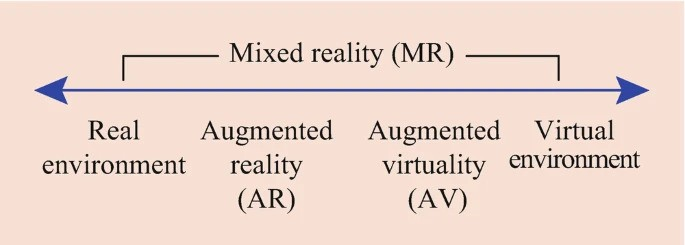
\includegraphics[width=0.5\linewidth]{dissertation//images/rvContinuum.jpg}
    \caption{Diagram of the Virtual Continuum, taken from \citep{vertucci_history_2023}}
    \label{fig:rvContinuum}
\end{figure}

In 1999, Hirokazu Kato developed ARTookKit. This is an open source library which can track the rotation of a camera in real time using markers \citep{kato1999marker}. This was revolutionary in the field of AR as research was still unable to find a good way to track the direction a user was looking. ARToolKit is still used in platforms such as Unity today \citep{vertucci_history_2023}.

Since the 2000s, there has been rapid growth in processing power, especially in smaller, mobile devices. This has allowed AR development to improve exponentially. A multitude of AR applications have been developed for handheld devices. This includes the first handheld AR application on a PDA, created by Daniel Wagner and Dieter Schmalstieg \citep{1241402}. In 2005, the ARToolKit was ported to allow development of AR on mobile devices \citep{10.1145/1179849.1179865}. In 2008, the first AR web browser was released by Mobilizy \citep{vertucci_history_2023}. In 2013, Google released the Google Glass which enabled users to view content through glasses \citep{vertucci_history_2023}. In 2016, Microsoft released a product which improved on almost every aspect of the Google Glass, the Hololens \citep{vertucci_history_2023}.

Since then, AR tools have become more standardised for developers to create AR apps across multiple platforms. This change has been heralded by SDKs provided by Apple and Google. ARKit by Apple is an SDK designed to create AR applications for iOS. 
It comes with features such as environment tracking, image tracking, face tracking and more \citep{9204243}. ARCore is Google's answer to ARKit. It works across a range of devices including Android and iOS devices. It's features are mostly similar to that of ARKit \citep{9204243}. These platforms open up the opportunity for problems with an effective AR solution to be easily implemented and be accessible across most modern mobile devices.

% Consider discussing relevant AR terms e.g. three tracking categories
% Perhaps more about HMDs

Today, the market for AR specific devices for consumers is beginning to form. This has taken the shape of head mounted displays. The Microsoft Hololens 2 \citep{microsoft_hololens_2019} released in 2019 with a focus on being used for industrial purposes.After this, the Apple Vision Pro \citep{apple_apple_2024} released in February 2024 with a marketing focus on the consumer. Head mounted displays offer a hands free alternative to smartphone AR for consumers

\section{Industrial Use of AR}

With the first use of the term augmented reality being for the use case of helping with assembling airplanes \citep{caudell1992augmented}, it is clear that industry is a key area in the advancement of AR technology. Since then, AR has been researched and used in a range of different industrial contexts.

\citet{Tang2004} found that using 3D AR instructions reduced error rate by 82\% for an assembly task. This was found through an experiment to test the effectiveness of AR assisted assembly in an industrial manufacturing environment. The experiment consisted of testing the effectiveness of AR instructions on a head-mounted display compared to paper instructions and computer-based instructions on a monitor \citep{Tang2004}. \citet{upskill_upskill_2017} gave a worker in a warehouse new picklist orders through an AR display which resulted in the process being 46\% faster than the regular operation.

\citet{wu_cognitive_2023} puts forward the idea of using wearable AR technology as a way to improve productivity in the field of construction. An AR application was designed that would guide construction workers on tasks and provide real-time information. It offered features such as 3D animations, translucent 3D representations of objects with x-ray vision, live warnings and more \citep{wu_cognitive_2023}. This was tested with two groups, one using paper instructions and another using the Hololens AR application. Participants completed a rebar-tying task and metrics such as time, quality and subjective experience was measured as shown in figure \ref{fig:arConstruction} \citep{wu_cognitive_2023}. 

\begin{figure}[hbt!]
    \centering
    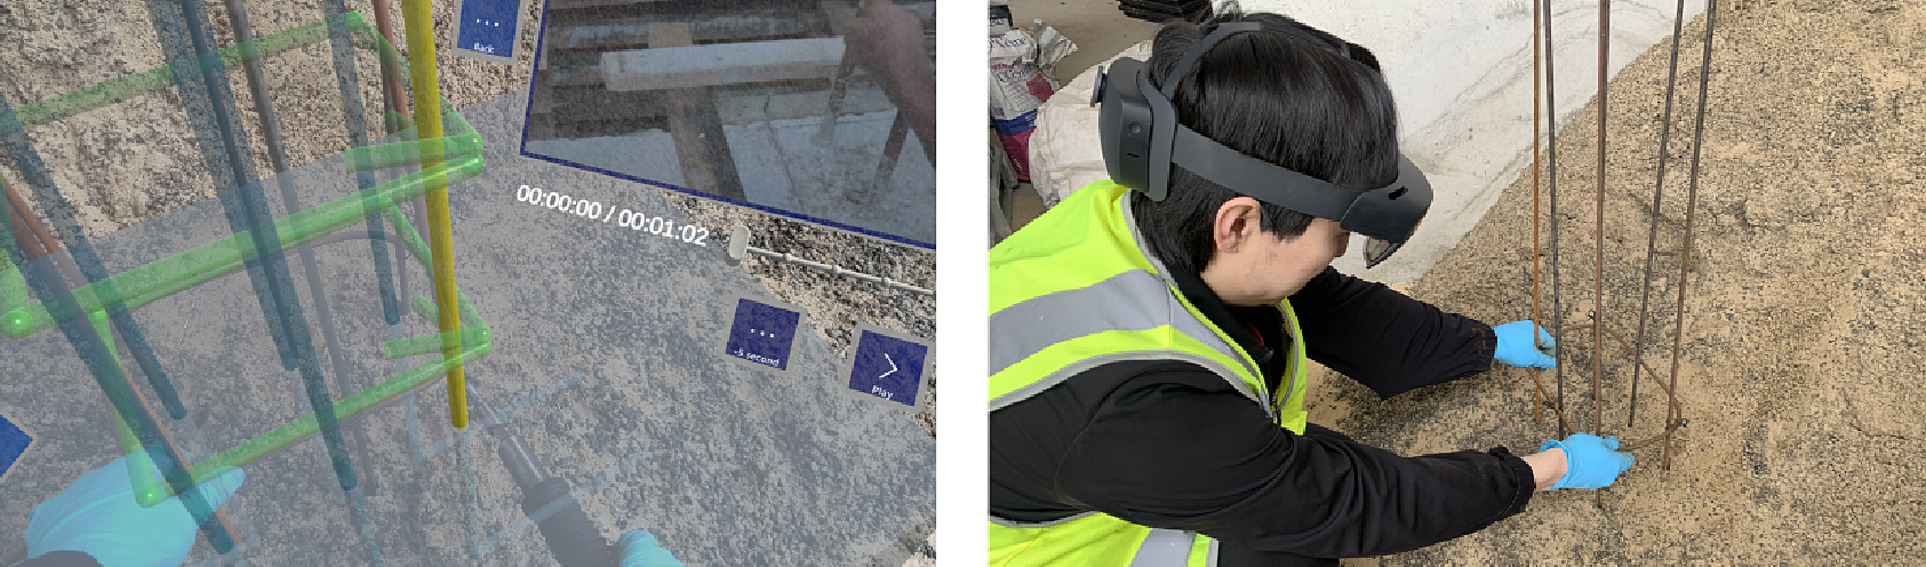
\includegraphics[width=0.8\linewidth]{dissertation//images/arConstruction.jpg}
    \caption{The AR construction application by \citet{wu_cognitive_2023} in use in an experiment}
    \label{fig:arConstruction}
\end{figure}

Results from the experiment found that the AR application significantly improved performance and understanding. Using the AR application improved kinaesthetic performance by around 40\% \citep{wu_cognitive_2023}. AR participants experience less frustration despite a similar amount of physical strain than the other group as they could quickly find information they needed for the tasks \citep{wu_cognitive_2023}. While \citet{wu_cognitive_2023} highlights that more research still needs to be done in the field, it emphasises the potential of the technology and the clear improvement it provides in productivity.

AR has proven to be a useful tool for workers in an industrial environment. A number of tests and studies have shown how effective it can be improving the productivity and experience of a worker, especially with manufacturing and assembly tasks. Despite the clear and great potential, the implementation of AR technology in manufacturing is not at the point it could be \citep{jalo_state_2021}.

\section{AR For Instructions}

With the success of using augmented reality for industrial purposes, research is being put into transferring the advantages to commercial use cases. The proven increase in productivity and reduction of error rates in industrial AR assembly tasks make for transferable benefits in AR tools for consumers. Many different types of product come with some sort of assembly requirement with provided instructions. Some of these products include furniture, home appliances, exercise equipment and outdoor equipment. This concept can also apply to products where assembly is a motivating factor in the purchase decision such as DIY model kits and \textit{LEGO} sets.

\citet{blattgerste_comparing_2017} tested the suitability of AR in providing assistance in different tasks. The focus of the study was on testing a range of devices and paper instructions on a Lego assembly task. There were three devices used in the study, a smartphone, a Microsoft Hololens and an Epson Moverio BT-200. Instructions were implemented into these devices and split into two groups. The smartphone and Hololens used instructions which placed a representation of the next block to be added in its correct location. The Epson Moverio BT-200 displayed pictures of the paper instructions to the view of the user \citep{blattgerste_comparing_2017}. The number of errors, cognitive load and task completion times were measured across instruction systems. Each participant carried out all four instruction methods \citep{blattgerste_comparing_2017}. Feedback from the experiment was generally negative towards the AR instructions. Handling the smartphone while trying to assemble was described as a difficulty. The pictures on the screen of the Epson Moverio BT-200 were too obstructive. The Hololens field of view was too small \citep{blattgerste_comparing_2017}. Despite the issues, one aspect that was commented positively on was the 3D placement of objects in the world, especially on the Hololens. Participants commented that it made sense and felt natural. They also described their appreciation of the hands-free nature of this option \citep{blattgerste_comparing_2017}. 

\citet{yang_comparing_2020} Conducted a very similar study by comparing paper to AR instructions on a Lego assembly task. Participants were split into two groups for paper and AR instructions. The AR instructions were on an Android app on a tablet. The app was created using Unity and Vuforia \citep{yang_comparing_2020}. Each group completed a set of training and experimental instructions, with the training set using a different model to the experimental set \citep{yang_comparing_2020}. The experiment measured effectiveness, efficiency, cognitive load and motivation. The study found that the effectiveness was improved on the AR instructions over the paper counterpart. This means that overall error rate was lower in AR \citep{yang_comparing_2020}. Within the qualitative feedback, participants reported that while the paper instructions were clear and easy to understand, the AR instructions felt intuitive and attractive \citep{yang_comparing_2020}. An interesting feature of the AR instructions was an animation function which shows the path of adding a part. Participants thought this was a helpful feature, "it shows the assembly path, so you can easily understand where bricks come from and how two bricks are connected." \citep{yang_comparing_2020}

\citet{chen_papertoplace_2023} created a tool for converting paper instructions to AR versions named PaperToPlace. The tool consists of two sections, a tool for authors to convert existing instructions to an AR format and an instruction viewing experience which dynamically places instructions in ideal locations \citep{chen_papertoplace_2023}. User studies were conducted for both sections but this research will focus on the results of the instruction consumption section. The study tested whether the AR instructions allowed users to complete tasks more efficiently and easily. Participants were given unfamiliar tasks and asked to complete them. Effectiveness was measured using performance analysis, a questionnaire and interviews \citep{chen_papertoplace_2023}. Results found that participants believed the tool made them work faster and easier. Switching contexts required less effort, with less head movement. Hands-free use was appreciated by the participants \citep{chen_papertoplace_2023}.

Bringing the innovations made in industry to the commercial market has proven to be fairly successful for users. AR is a tool which research shows, has an ability to improve user's performance in assembly tasks. Following from this, it is important to analyse whether there is a precedent for the use of AR in the case of flatpack furniture manufacturers and if it could be a commercially viable endeavour. 

\section{IKEA AR Apps}

An example of an AR product available to the public market currently is IKEA Place. The app, which launched in September 2017, offers users the ability to place IKEA products in a 3D, real life environment with an accurate scale. This means that users can gain an impression of how a piece of furniture will look in the context of their own surroundings without having to purchase and return a product. IKEA Place offers a 98\% accuracy on setting the scale of a piece of furniture \citep{ikea_launch_2017}.

\begin{figure}[hbt!]
    \centering
    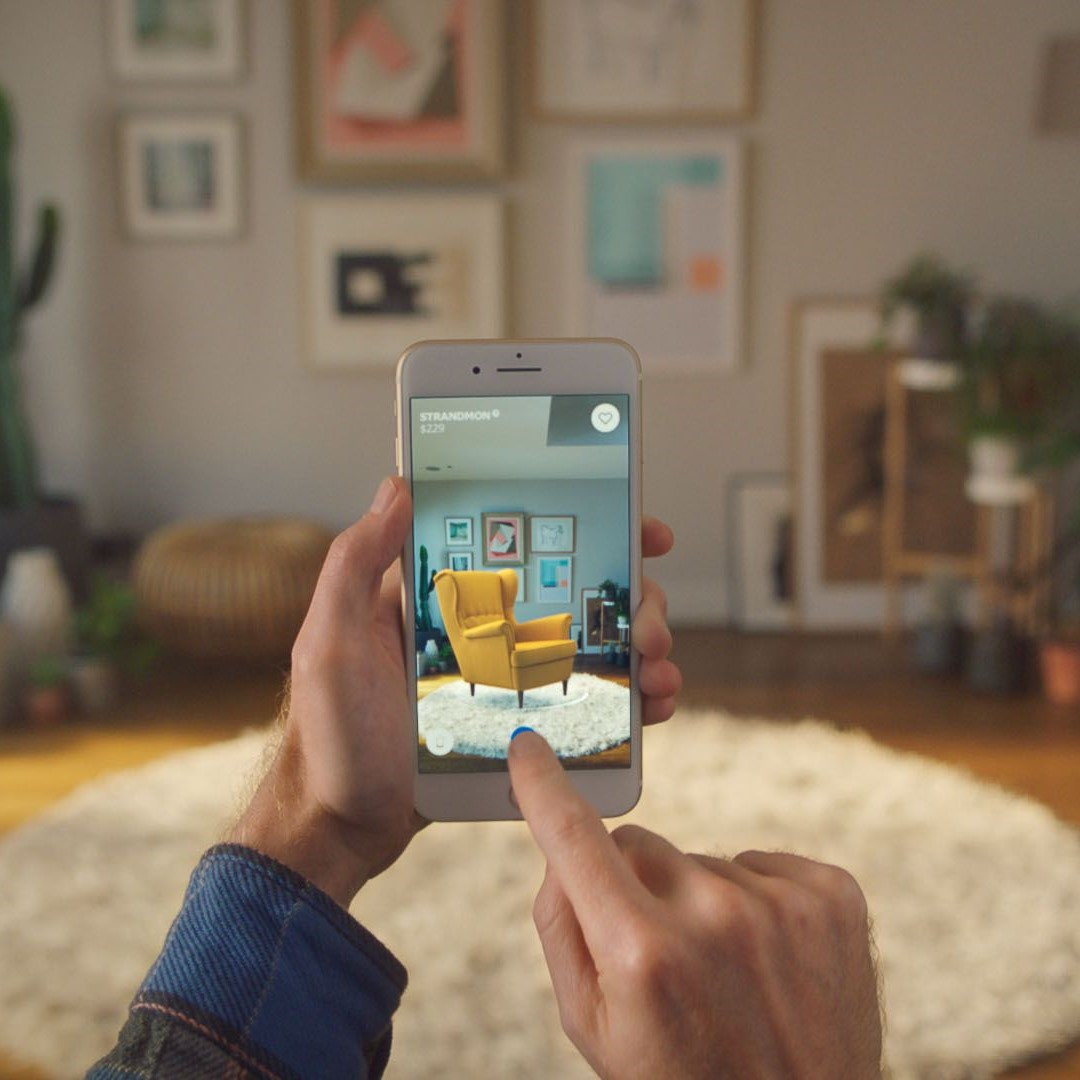
\includegraphics[width=0.5\linewidth]{dissertation//images/IKEAPlace.jpg}
    \caption{Demonstration of the IKEA Place app in use. \citep{ikea_launch_2017}}
    \label{fig:ikeaPlace}
\end{figure}

\cite{raska_influence_2017} conducted a study to determine if using an IKEA AR application increases a customers intent to purchase compared to using a product website. The study aimed to provide answers to marketers on how effective AR can be as an option to impact consumer behaviour. In particular, it wanted to know the effect an AR application has on a customers purchase intention, and assuming a positive effect was found, the cause of the effect \citep{raska_influence_2017}. To conduct this study, multi-method quantitative research was harnessed in the form of collecting data and a questionnaire \citep{raska_influence_2017}. In terms of data collection, primary and secondary sources were employed. Secondary data was gathered online using keywords to find relevant literature but it was determined that there was not enough pre-existing data in this field. For this reason, primary data was gathered to provide insights into which factors affect a consumers purchase intentions \citep{raska_influence_2017}. 

An experiment was set up to determine the causal relationship between AR and purchase intention. An experimental group were made to use the IKEA AR app in a simulated home environment. They were then instructed to take an online questionnaire. The control group were given the questionnaire alone. The design of the questionnaire involved a rating scale and aimed to determine attitude towards IKEA products and AR technology \citep{raska_influence_2017}.

From the testing on 177 participants, it was found that purchase intention was higher in the experimental group, suggesting that the experience of the AR product increased enjoyability and was useful \citep{raska_influence_2017}. Despite this, similar levels of attitude towards the AR app were recorded between groups \citep{raska_influence_2017}. The study concludes that AR technology can positively influence purchase intention, contradicting previous suggestions that AR may just be a gimmick. It suggests that companies should hone in on improving their AR applications, especially with the introduction of more open platforms \citep{raska_influence_2017}.

From this we can gather that using AR technology has potential to improve the performance of a business, especially in the case of IKEA or other ready-to-assemble furniture companies. With an emphasis being placed on businesses focusing on and expanding their AR capabilities, there is good reason to look deeper in to AR in the field of flatpack furniture. % If we need more look to source "Service innovation..."

\section{Flatpack Furniture}

Flatpack furniture, also known as ready-to-assemble furniture (RTA), provides a cheaper alternative to furnishing a space than pre-assembled furniture. The customer receives a flat box full of parts with a set of instructions. They then are required to follow the instructions to assemble the furniture themselves \citep{fleming_ritsy_nodate}. The concept for flatpack furniture came about in the early 20th century when Louise Brigham tried to popularise her idea for ready-made box furniture \citep{lafarge_ready--assemble_2019}. Despite this, the idea for RTA only gained widespread recognition later in the mid-20th century with different businesses being established in the 1950s \citep{lafarge_ready--assemble_2019}. Many of the inspirations for starting a RTA business stem from a lack of affordable furniture options for working class people \citep{lafarge_ready--assemble_2019}. Nowadays, companies like IKEA dominate the market with their flatpack furniture options.

Despite the longstanding popularity of flatpack furniture, people still have difficulty assembling their own products. According to a study in 2007 by Miles Richardson, 67\% of adults had difficulty in assembling flatpack furniture, out of a 52\% that had assembled in the previous two years. 13.8\% of these people claimed to have damaged the furniture they were assembling and a further 7.8\% of people say they ended up with some form of injury from the assembly process \cite{Richardson11}. With such a high percentage of people having trouble with these assembly tasks, it leaves a gap for research to find a definitive solution to this problem.

\section{Gap In Research}

Augmented reality has become a very large field in the last two decades. It is being proven to be an effective tool in manufacturing and assembly for industrial purposes. The benefits of this are also being harnessed in providing instructions and guidance to users of commercial products. Along with this it is also being used in the specific case of flatpack furniture to provide IKEA customers with a view of how a piece of furniture will look and fit in a particular space. This has proven to be a valuable and effective venture for IKEA. 

Flatpack furniture is a popular solution to providing those who require it, quick and cheap furniture. The issue is that many people struggle with the task of assembling the furniture. Research to finding a solution to this is vital and the proven benefits of AR offer a potential path to finding one.

Studies which look to the use of AR to help with the assembly of flatpack furniture have been conducted. \citet{hartanto_development_2019} shows the creation of an application which used AR to guide users with manipulable and interactable tools. The application, named ARSembly, worked on android devices and was tested using a questionnaire \citep{hartanto_development_2019}. While the results did show positive feedback for the product, there are a few issues with the research. Firstly, the user study is not particularly well designed. A random 50 users of the app were selected to respond to the questionnaire \citep{hartanto_development_2019}. No in-person or live trials were conducted on the app's effectiveness. The AR instructions were never directly compared to paper instructions, the only comparison is through the response to a question that showed that most users found it easier to use than paper instructions \citep{hartanto_development_2019}. The question this data comes from is not particularly clear as the questions are not directly given, only tables of the results with explanations of the theme of the question. It is not confirmed if respondents were even instructed to compare this against paper instructions. Overall, this research is very weak and unreliable. The questionnaire is not strong enough evidence to prove the effectiveness of this method in the field of flatpack furniture. Furthermore, this research uses an application on a phone as the base of the study. A head mounted display is better for completing tasks, especially due to the hands-free nature, as shown in \citep{blattgerste_comparing_2017, chen_papertoplace_2023}.

More research needs to be conducted in this field. The previous literature point towards AR instructions on a head mounted display being a strong contender for improving the experience of assembling flatpack furniture. There is a lack of significant research to prove or disprove this potential.

%==================================================================================================================================
\chapter{Analysis/Requirements}
\label{chap:analysis}

\section{Analysis of Problem}

An AR solution to flatpack furniture instructions is required in the problem. These instructions are commonly paper-based and give a picture-by-picture guide to assembling the furniture, as shown in figure \ref{fig:instructions}. Taking this to the world of augmented reality opens up a plethora of opportunities. AR takes digital content into the real 3D world and is much more dynamic and fluid than the 2D paper methods.

Creating a new AR platform to communicate instructions on assembling flatpack furniture to a user requires the translation of certain concepts into an AR environment. For this to be done effectively, a user must be able to fully follow through with the instructions without any outside help or guessing. To ensure that this is the case, a set of requirements have been created for the platform to follow.

\section{Functional Requirements}

\subsection{Requirements from Paper Instructions}

It was important to analyse the paper instructions provided with a set of flatpack furniture to understand the baseline that the AR instructions would be compared to. The paper instructions for the IKEA HEMNES bedside table \ref{fig:instructions} were inspected to find the most important factors in helping a person assemble furniture.

\begin{figure}[hbt!]
    \centering
    \includegraphics[width=1\linewidth]{dissertation//images/instructions.jpg}
    \caption{Paper instructions for IKEA HEMNES bedside table \cite{noauthor_hemnes_nodate}}
    \label{fig:instructions}
\end{figure}

The paper instructions provide a good guide on the order steps should be completed in. The AR instructions should follow this structure and order to ensure that the furniture is assembled correctly.

% If needed, add breakdown of steps as list here
The main steps covered in each page include:

\begin{enumerate}
    \item Adding the rails for the drawer to each set of legs and adding screws to each set of legs to connect them to the rest of the parts.
    \item Adding the back board and under drawer connector to one set of legs and tightening the connection of the new parts to the legs.
    \item Installing the shelf in the middle of the legs, tightening the connection and adding the second set of legs to the rest of the assembly.
    \item Tightening the connection between the second set of legs and the rest of the assembly, adding foot pieces to the bottom of the legs and adding dowels to prepare for the addition of the top shelf.
    \item Installing screws to the top shelf to connect it to the rest of the assembly and tightening the connection between the top shelf and the rest of the assembly.
    \item Adding screws to the front of the drawer to connect it to the side pieces, installing both side pieces and tightening their connection.
    \item  Sliding in the bottom of the drawer, adding the back of the drawer and screwing it to the sides.
    \item Pulling out the rails and sliding the drawer in.
    \item Adding a screw to the front of the drawer and screwing in the handle.
\end{enumerate}

There are a few important techniques used in these instructions that can be carried over as functional requirements for the AR instructions. To prioritise which requirements are the most important to be implemented, the MoSCoW method was used \citep{business_chapter_2024}. Requirements are either labelled must have, should have, could have or won't have this time. These features are key to making it clear to a user how to progress in assembly. The requirements gained from assessment of the paper instructions include:

\begin{itemize}
    \item Covering all of the steps to complete the assembly (must have)
    \item Identifying which new part should be added (must have)
    \item Making it clear where a part goes (must have)
    \item Showing the path a part should be added in (should have)
    \item Showing the orientation a part should be added in (must have)
    \item Communicating if a component needs to be assembled separately then added to the full assembly after (must have)
    \item Declaring when a part should be screwed in (should have)
    \item Giving a position to place the work in progress assembly when adding a new part (should have)
    \item Showing a close up view of smaller parts (could have)
    \item Always having access to a view of the finished product (should have)
\end{itemize}

\subsection{Requirements of Augmented Reality}

The nature of completing this task using AR technology means that the application should implement particular features that AR uniquely offers. 

\begin{itemize}
    \item Users must be able to view parts from any angle (must have)
    \item There should be a way to show that a part is in the right place (should have)
    \item The assembly must be placed in the user's environment (must have)
    \item The assembly must stay in the same place during a step (must have)
    \item Users should be able to tell where, in their environment, the assembly currently is (should have)
    \item The scale of every 3D object must be accurate to reality (must have)
    \item The form of every 3D object must be accurate to reality (must have)
\end{itemize}

\section{Non-Functional Requirements}

Adding on to the functional requirements, non-functional requirements were set. These are requirements that the system should have.

\subsection{Hardware Requirements}

Microsoft's Hololens 2 is the chosen platform for this task. Due to this there are particular requirements it must follow to be compatible. 

\begin{itemize}
    \item The application must be able to built to the Hololens 2 (must have)
    \item The application must run well on the Hololens 2 (must have)
    \item The application must only use features which are available on the Hololens 2 (must have)
\end{itemize}

\subsection{Software Requirements}

The system must follow certain requirements to ensure that is can be expanded upon for potential future use.

\begin{itemize}
    \item The system must be modular to allow for new part/instruction types to be added (must have)
    \item The system should automatically read in new 3D models to set up new instructions (should have)
\end{itemize}

%==================================================================================================================================
\chapter{Design}
\label{chap:design}

\section{Instructions System Architecture}

One of the most important goals of the project was translating a set of paper instructions to a digital, 3D format. A system was required that broke a piece of furniture up into each of its parts which would then be added in a particular step. The system would contain all of the required information about each part and step which could then be taken and visualised in the engine used.

The system utilised the composite design pattern \citep{riehle_composite_1997} as a foundation, while also tailoring the implementation to suit the unique requirements of the application. In a furniture assembly, there are parts and there are components which are made up of other parts and then added as parts themselves. This idea can be represented as a tree structure as shown in figure \ref{fig:compPattern}. 

\begin{figure}[hbt!]
    \centering
    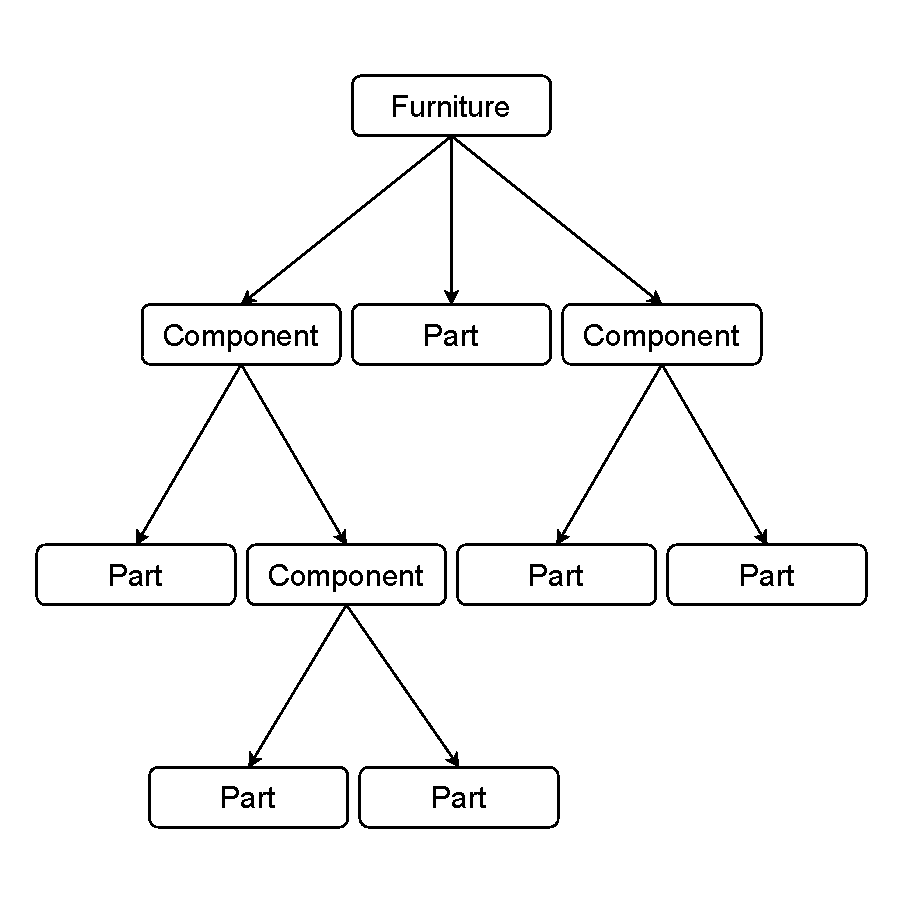
\includegraphics[width=0.5\linewidth]{dissertation//images/compositePattern.pdf}
    \caption{A representation of the parts of an assembly in tree form which shows how the composite pattern can be utilised in this scenario.}
    \label{fig:compPattern}
\end{figure}

Components can be broken up into a group of parts or other components. Parts are considered the leaf node of the tree. Using this system means that, if required, new types of parts could be added and fit in the tree as long as they inherit the correct object. The system separates from the composite design pattern as nodes in the tree do not implement one common interface, instead they all inherit the part object to receive their common methods as shown in figure \ref{fig:classDiagram}.

\begin{figure}[hbt!]
    \centering
    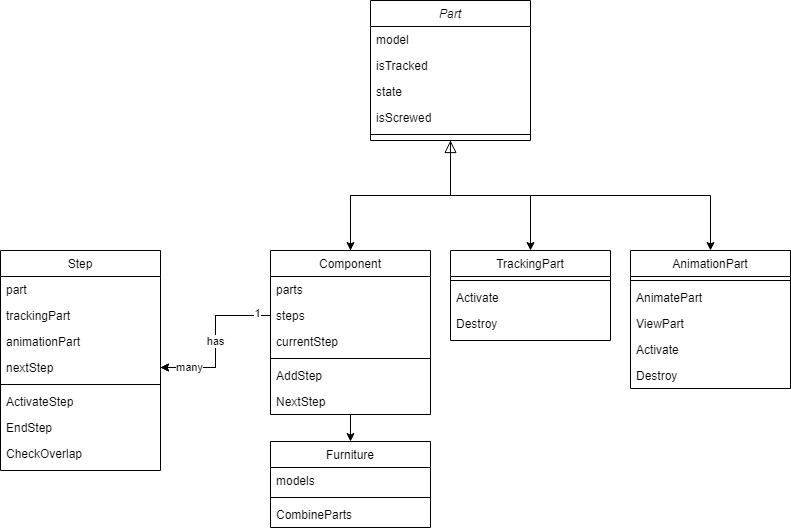
\includegraphics[width=0.8\linewidth]{dissertation//images/classDiagram.jpg}
    \caption{Class diagram showing the set up of the instructions system}
    \label{fig:classDiagram}
\end{figure}

% Maybe add parent position and rotation to Part ^^^

The system in figure \ref{fig:classDiagram} is designed to step through parts in the order of the instructions. \textit{Furniture} is the base object that will be created in the engine. As a child of \textit{Component} it has a list of parts which can either be a \textit{Part} or \textit{Component}. It is provided with models which are set up in a particular way, as shown in chapter \ref{modelSetup}, which allows it to convert each model to a \textit{Part} or \textit{Component} and put them in the correct order into the parts list. If a model is standalone with no children, meaning it should just be added to the assembly by itself, it is a \textit{Part}. If the model has children, meaning it should be assembled separately then added to the full assembly, it is a \textit{Component}. For each item in this list there is also a \textit{Step} or list of steps. Each \textit{Component} has a list of steps and a current step. A \textit{Step} has a \textit{Part}, \textit{TrackingPart}, \textit{AnimationPart}, and a \textit{Step} which points to the next \textit{Step} in the order of the instructions. The AddStep function adds a \textit{Step} to the list based on a given \textit{Part}/\textit{Component} and automatically determines which type it is. For a \textit{Part} it will simply add a new \textit{Step} and set it as the nextStep of the previous one. For a \textit{Component} it will set the nextStep of the previous \textit{Step} to the first \textit{Step} of the \textit{Component} and the final item of its steps will point to a new \textit{Step} created for the \textit{Component} itself. A \textit{Part} has a model which would exist in the world space. It can either be tracked or animated and it can be screwed in. It has a state which can be either disabled, waiting, correct or finished. These represent the progress through a step of the instructions. If a \textit{Part} is tracked then its corresponding \textit{Step} will use a \textit{TrackingPart}, otherwise it will use an \textit{AnimationPart}. A \textit{TrackingPart} will automatically be connected to the object tracking system when created and will track its real life counterpart. An \textit{AnimationPart} automatically starts animating the motion of adding the part when created. The ActivateStep and EndStep methods of \textit{Step} will choose the right type of part to create and destroy when the step is active.

\section{Object Tracking}

The biggest feature of the application is showing the user how to add a part to the assembly. It was important that this was designed in a way that took advantage of the AR environment. The first chosen method to demonstrate a step was to track the parts in real life using the camera and a 3D model tracker. When an object is detected in the camera view, an overlay of the 3D model in red is displayed in the same position. The same model is also displayed in the position it should be placed in a blue colour. When the real part is tracked to be in the same position and rotation as is required then it is turned green to show that it is correct.

\section{Animation Visualisation}

The second method chosen to demonstrate how to carry out a step was by using animations. One of the 'should have' requirements was to show the path that a part should be added in. This means that the application should demonstrate to a user the optimal way to move a part into the correct position. \citet{yang_comparing_2020} found in a study that participants described this as a helpful feature for a Lego assembly task. 

In this case, the current part is created at a start point and travels towards the correct location. When it reaches the correct location and rotation it turns green and waits briefly. It then gets set back to the original position and repeats the process again. The starting position and rotation are carefully set in order to demonstrate, during the animation, the best way to add the part.

\section{Appearance}

To highlight the state of parts in each step, particular colours and materials were chosen with different meanings. The positioning of parts at each step can also have a meaning. Parts which have not been reached yet are displayed in a very transparent white material. They are shown in the correct place in relation to the rest of the assembly. This allows users to be able to see the completed assembly at any point, as described in one of the requirements, without it obstructing the view of the current step. Parts which have already been added are shown in an opaque white colour in their correct location to demonstrate the current progress of the assembly. Focusing on an active step, there are two versions of the current part, one which is always in the correct location and one which is tracked or animated. The part in the correct location is set to a semi-transparent blue colour which helps it to stand out and show the user where they are meant to add the part. The tracking/animation part is shown in a semi-transparent red colour while it is not in the correct location. When these two part types meet in the correct location, they both turn to a less transparent green colour to make clear that the part has been placed correctly.

Extrapolating from this, it is clear that the position and appearance represent five different internal states that parts can hold:

\begin{enumerate}
    \item \textbf{DISABLED} - The part is not in use yet.
    \item \textbf{WAITING} - The current part is waiting to be reached by the tracking/animation part.
    \item \textbf{TRACKING/ANIMATING} - The tracking/animation part is waiting to reach the correct location.
    \item \textbf{CORRECT} - The tracking/animation part and the current part to be added have both met in the final position.
    \item \textbf{FINISHED} - The part has been added to the full assembly
\end{enumerate}

\section{Other Features}

Other features were designed in response to some of the requirements. One of the `should have' requirements is that the user should be able to tell where the assembly currently is. In an augmented reality environment, the user is able to look around 360 degrees and is also able to move around the environment. This means that a user could potentially lose sight of the current step. In order to counteract this issue, a pointer was planned to point the user back on track. If the location of the current step is outside of the user's field of view then an arrow appears on screen that points in the direction of the step.

Another `should have' requirement was that the application should indicate when a part should be screwed in. To make clear to the user when a part needs to be screwed in, an indicator was designed. Arrows to indicate rotation should be placed around the location of a screw part. They should rotate in the correct direction around the centre point of the screw hole.

\section{Model Setup} \label{modelSetup}

In order to visualise the system there had to be 3D models for each part of the assembly. Each model had to be accurate and positioned correctly relative to the other models. In order to accomplish this a template was designed which would automatically integrate with the instructions system. 

\begin{figure}[hbt!]
    \centering
    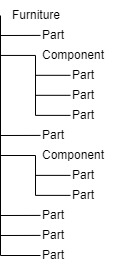
\includegraphics[width=0.2\linewidth]{dissertation//images/modelFileStructure .jpg}
    \caption{Example model structure to be provided to the instructions system}
    \label{fig:modelStruct}
\end{figure}

Each part is an individual 3D model which can be grouped together to make a component or left alone. All components and parts are then grouped to the full furniture model and positioned correctly. Once this model is correct, a list of each part and component is created which is ordered in the order of when parts are added. The list also contains a position and rotation which the parent of a part should be moved to while the part is being added.


%==================================================================================================================================
\chapter{Implementation}
\label{chap:implementation}

\section{Choosing Unity as a Development Platform}

Selecting an appropriate development platform was a pivotal step in ensuring a successful project. It was required that the platform was capable of certain features from the start. 3D rendering was a necessary capability. It was imperative that AR development was possible on it without too much difficulty in set up. Features that made building to the Hololens an easy process were also important.

In this case, Unity was the best choice for a development platform. Unity is an extremely versatile platform. At a base level it comes with capabilities to easily set up a project and render in 3D. Unity uses a system which encourages adding packages based on what the project is. It has a range of AR packages, provided by Unity, which can be installed in a click using the package manager window. Any other packages required can be installed from the same window using a link or download file. The project benefits from being able to use the enhancements provided by external packages which can be easily integrated in Unity.

Moreover, Unity was the first choice based on prior experience gained in development of other projects. Having previous experience in Unity development with projects of a similar nature, including AR projects, familiarity of the functionality and features allows for a significantly smaller learning curve than trying to learn a new platform. This allows for a more efficient workflow and more time that can be dedicated to development. Unity uses C# as its development language. This has been used in previous projects which means the project will be written in a familiar language. Choosing Unity results in a stronger final project due to the extra time and higher quality implementation.

The selection of Unity as the development platform was a clear decision informed by prior experience, technical suitability and versatility. These factors allow the project to reach the requirements at a high standard in a suitable amount of time.

\section{Tracking Method}

Object tracking was an important part of the project design. Objects, such as parts of the furniture, were to be tracked in the camera view. These parts had to be accurately tracked in real time in order to verify the placement and highlight errors to users. This is a very complex task and requires the right framework for it to be done effectively. A selection of different options for this test were reviewed and tested.

\subsection{Unity Image Tracking}

One of the packages available to install in Unity is AR Foundation. This package comes with many different augmented reality capabilities such as device tracking and image tracking as shown in table \ref{tab:arfFeatures}. 

Image tracking is a particularly useful feature for this project. If unique images are placed on each part in real life and then matched up in Unity, this could be used to track their position. This feature was tested with a very small prototype. Three QR codes were printed off at three different sizes, small to large. A Unity project was created that placed a 3D model on the QR codes and when this was tested on an Android phone, it proved to be very effective at each size of QR code. Unfortunately, if image tracking were to be used, images would have to be placed all over each part of the furniture, which is not a particularly realistic set up for flatpack furniture.


% Please add the following required packages to your document preamble:
% \usepackage{multirow}
\begin{table}[hbt!]
\caption{List of available features across all Unity supported AR platforms. \cite{noauthor_ar_nodate}}
\label{tab:arfFeatures}
\centering
%\tt 
\rowcolors{2}{}{gray!3}
\begin{tabular}{|l|c|cc|cc|}
\hline
\multicolumn{1}{|c|}{\multirow{2}{*}{\textbf{Feature}}} & ARCore           & \multicolumn{2}{c|}{ARKit}                            & \multicolumn{2}{c|}{OpenXR}                                  \\ \cline{2-6} 
\multicolumn{1}{|c|}{}                                  & \textbf{Android} & \multicolumn{1}{c|}{\textbf{iOS}} & \textbf{visionOS} & \multicolumn{1}{c|}{\textbf{Hololens}} & \textbf{Meta Quest} \\ \hline
Session                                                 & Yes              & \multicolumn{1}{c|}{Yes}          & Yes               & \multicolumn{1}{c|}{Yes}               & Yes                 \\
Device Tracking                                         & Yes              & \multicolumn{1}{c|}{Yes}          & Yes               & \multicolumn{1}{c|}{Yes}               & Yes                 \\
Camera                                                  & Yes              & \multicolumn{1}{c|}{Yes}          &                   & \multicolumn{1}{c|}{}                  & Yes                 \\
Plane Detection                                         & Yes              & \multicolumn{1}{c|}{Yes}          & Yes               & \multicolumn{1}{c|}{Yes}               & Yes                 \\
Image Tracking                                          & Yes              & \multicolumn{1}{c|}{Yes}          & Yes               & \multicolumn{1}{c|}{}                  &                     \\
Object Tracking                                         &                  & \multicolumn{1}{c|}{Yes}          &                   & \multicolumn{1}{c|}{}                  &                     \\
Face Tracking                                           & Yes              & \multicolumn{1}{c|}{Yes}          &                   & \multicolumn{1}{c|}{}                  &                     \\
Body Tracking                                           &                  & \multicolumn{1}{c|}{Yes}          &                   & \multicolumn{1}{c|}{}                  &                     \\
Point Clouds                                            & Yes              & \multicolumn{1}{c|}{Yes}          &                   & \multicolumn{1}{c|}{}                  &                     \\
Raycasts                                                & Yes              & \multicolumn{1}{c|}{Yes}          &                   & \multicolumn{1}{c|}{Yes}               & Yes                 \\
Anchors                                                 & Yes              & \multicolumn{1}{c|}{Yes}          & Yes               & \multicolumn{1}{c|}{Yes}               & Yes                 \\
Meshing                                                 &                  & \multicolumn{1}{c|}{Yes}          & Yes               & \multicolumn{1}{c|}{Yes}               &                     \\
Environment Probes                                      & Yes              & \multicolumn{1}{c|}{Yes}          &                   & \multicolumn{1}{c|}{}                  &                     \\
Occlusion                                               & Yes              & \multicolumn{1}{c|}{Yes}          &                   & \multicolumn{1}{c|}{}                  &                     \\
Participants                                            &                  & \multicolumn{1}{c|}{Yes}          &                   & \multicolumn{1}{c|}{}                  &                     \\ \hline
\end{tabular}
\end{table}

Furthermore, the image tracking feature is unavailable on Hololens. If this feature were to become available it would certainly be a good option for this project.

\subsection{Azure Object Anchors}

Object Anchors is a Microsoft Azure service for tracking 3D models in real space. Azure Object Anchors is an SDK specifically designed for use on the Hololens. It works by uploading a 3D model to the Azure servers which then return a converted Azure Object Anchors model. This model is stored on the Hololens and is used for tracking. 

There are many drawbacks to using Object Anchors. One of which is that using the service costs money. There are a set amount of student credits available but the pricing of use was unclear. Another issue is that Object Anchors does not support tracking moving objects which would hinder a users ability to get a live idea about when they have a part in the correct location. When tested using a custom 3D model, the tracking proved to be very difficult to use.

\subsection{VisionLib}

VisionLib is a library developed for augmented reality model tracking created by Visometry \citep{visometry_visionlib_nodate}. VisionLib can be used across multiple platforms including Unity and Unreal Engine. When used in Unity, if the scene is set up correctly, all VisionLib needs to start tracking a model is a game object with a mesh. This means that there are no restrictions on model formats, as long as they work in Unity, and there is no conversion process. It uses init poses to detect models. This means that models are displayed in a certain pose and when this pose is matched by the real counterpart, it begins tracking it. This is very useful for the case of this project as it allows parts to be clearly displayed to the user before it can be tracked to the correct location. % more probably

VisionLib requires a license to use. A trial license can be acquired that lasts 30 days but after this, Visometry must be contacted to seek a price for a full license.

\section{Licensing Troubles}
\label{sec:license}

Visometry was contacted to request a price to use VisionLib for this project. However, they offered a free 6-month education license for this occasion. They required certain details to set it up and the license had to be sent back. Unfortunately, when the license was sent by email, the email was blocked automatically, which was not immediately clear. On attempt to get access to the license using another method, it took 6 weeks to acquire. This caused significant issues for development. During this time, the object tracking method was switched to Azure Object Anchors, however it did not suit the project very well. Once the license was gained, development could get back underway but the consequences of this delay were that there was much less time to gain a full understanding of how to use VisionLib to its full effectiveness.

\section{Setting Up Project}

A Unity project was set up using the base 3D template on Unity version 2021.3.13f1. To prepare the project the VisionLib SDK was imported from the package manager. The application offers a part outlining feature which is not active in the final product but is still integrated into the scripts. The outline system was developed using the Quick Outline package from the Unity store \citep{nolet_quick_2022}. The Mixed Reality Feature Tool \citep{kerawala_welcome_2022} was used to import particular packages which are required for AR Hololens projects in Unity. Setting up Unity for building to the Hololens is a very tedious task, therefore a guide was used to set up the project settings properly \citep{qianw211_unity_2022}. VisionLib provides packages which import a selection of scenes which are pre-made for different purposes. For example, a multi-model tracking scene, a model switching scene and a Hololens model tracking scene. A copy of the Hololens model tracking scene was created as a base for this project.

The scene was set up with five top level objects \textit{VLTracking}, \textit{SceneContent}, \textit{Input}, \textit{XRRig} and \textit{Manager}.

\textit{VLTracking} was created in the VisionLib Hololens model tracking template and it handles setting up the tracking capabilities. This is where the provided license file is placed and also provides some different tracking paramaters which can be edited.

\textit{SceneContent} is where all of the tracking and animation parts are stored. It has the children objects \textit{VLTrackingAnchor} and \textit{AnimationParts}. Parts under \textit{VLTrackingAnchor} have tracking mesh scripts attached which means that VisionLib can use their mesh for tracking. These parts are all positioned in front of the camera in a precisely chosen pose as these are the init poses required to start tracking. Parts under \textit{AnimationParts} are used for animation instructions and are all set in the position their animation should start. \textit{SceneContent} also includes a light for the scene.

\textit{Input} contains the object which detects speech and keyboard input and points to the given command when input is received.

\textit{XRRig} contains the camera object. It includes a script which sets the floor level of the scene. This is done by setting a vertical offset for the camera which represents the distance of the Hololens to the floor at the start of runtime. This was set as close as possible to the eye level of the researcher to ensure consistency during testing.

\textit{Manager} contains a script which handles setting the scene up during runtime and connecting the scene to the instructions scripts.

\section{Custom Framework for Instructions}

The framework designed in figure \ref{fig:classDiagram} was implemented using C\# in Unity. 

Two extra scripts, \textit{Instructions.cs} and \textit{Manager.cs}, were created to integrate the instructions framework with the Unity editor. The manager script was attached to a permanent game object in the scene and was used to set up the scene properly in runtime. It also handled all of the input. The manager script handled instantiating the correct furniture prefab depending on if tracking or animation was being used. Furthermore, it set up their instructions script. Lastly, it would set the position and visibility of the pointer arrow in listing \ref{lst:arrow}.

The instructions script is used to transfer data from the Unity editor and properly set up the furniture object. When a game object contains the instructions script, it has a range of editable properties in the Unity editor shown in \ref{fig:properties}.

\begin{figure}[hbt!]
    \centering
    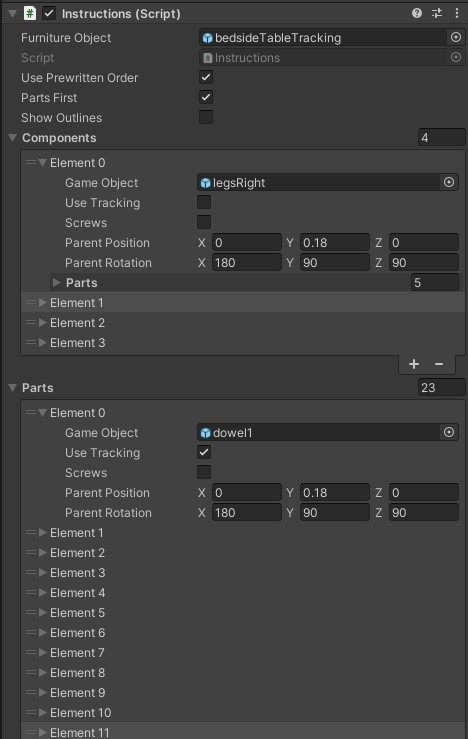
\includegraphics[width=0.4\linewidth]{dissertation//images/instructionsProperties.jpg}
    \caption{All of the editable properties for the instructions scripts.}
    \label{fig:properties}
\end{figure}

The editor contains a list of parts and components which are generated from the given furniture object, which is the top parent of the furniture model. These lists are generated using the InstructionsEditor.cs script. This script checks for a change to the furniture object field and creates a parts and components list based on the children of the new object. If a child is a parent itself, it is added to the components list, otherwise it is added to the parts list. This list is passed by the instructions script to the furniture object which combines it into one list to create all of the parts and components, it also creates all of the steps in the order of the list. A limitation of this system is that instructions must be in the order of either parts first or components first. Ideally, the editor could have one list which can contain parts and components, since they both inherit from part, however, the Unity editor by default does not support polymorphism in serialised lists. Solving this would require dedicating a large amount of time to creating a stronger editor or downloading a custom editor which can be costly. Instead, a workaround was created that exclusively works for the specific furniture used in this project. If the 'Use Prewritten Order' toggle is checked in the instructions script, the furniture object will detect if there is a recognised piece of furniture being used and then use another function to combine the lists. This function has a hard coded order to select parts and components from both the lists in the instructions script. Each selected item is then added to the furniture with a corresponding step being created in that order.

\section{Setup of Bedside Table Prefab}

% 2 prefabs were set up for animation and tracking
In Unity, a prefab is a game object that can be saved and reused in its exact form. The components and children of the game object are stored in the state they are saved at. They can then be newly instantiated into a scene and edits to their properties can be made.

Since the project was going to be tested using an animation version and a tracking version, two prefabs were created of the bedside table model with the instructions script attached. The properties of each prefab were almost exactly the same with the only difference between them being that the tracking prefab had 'Use Tracking' checked for particular parts. This meant that if the tracking option was selected at the start of runtime, the tracking prefab would be spawned and certain parts would use VisionLib tracking while the rest would use animation. If the animation option was selected then all parts would use animation.

The rest of the properties in each prefab were adjusted to suit the steps of the furniture assembly. Parts that had the 'Screws' toggle selected would be indicated on the screen that they were to be screwed in rather than just placed in. The 'Parent Position' and 'Parent Rotation' properties represent a 3D vector location and rotation for the parent of the current part to be in while the part is being added. This is useful for showing the user the ideal position to place the work in progress assembly during the current step.

\section{Input}

One of the features that comes with the VisionLib Unity package is Bluetooth keyboard and voice command input for the Hololens. It works as a component which can be added to game objects. New voice commands can be typed into the Unity inspector which can then be tied to a function of a script in a specified game object. These voice commands were harnessed as the primary input for using the program. Five new voice commands were created as shown in table \ref{tab:voiceComs}. These commands were also set up for keyboard use if required.

\begin{table}[hbt!]
\caption{The custom created voice commands for the project, the script and function they call and a description of their effect. It should be noted that these are separate from the default voice commands created in the VisionLib template set up.}
\label{tab:voiceComs}
\centering
\rowcolors{2}{}{gray!3}
\begin{tabular}{l|l|l}
Voice Command   & Script.Function           & Effect                                                                                                                           \\ 
\hline
"Use Tracking"  & Manager.SetUseTracking    & \begin{tabular}[c]{@{}l@{}}Initialises program to use the\\object tracking variation\end{tabular}                                \\
"Use Animation" & Manager.SetUseAnimation   & \begin{tabular}[c]{@{}l@{}}Initialises program to use the\\object animation variation\end{tabular}                               \\
"Start"         & Manager.StartInstructions & \begin{tabular}[c]{@{}l@{}}Starts the instructions using the\\specified mode\end{tabular}                                        \\
"Next Step"     & Manager.NextStep          & \begin{tabular}[c]{@{}l@{}}Moves the instructions on the the\\next step/part\end{tabular}                                        \\
"View"          & Manager.ViewPart          & \begin{tabular}[c]{@{}l@{}}For animated parts only, toggles the \\mode to get a~close up view of the\\current part\end{tabular} 
\end{tabular}
\end{table}

\section{Custom 3D Models}
% Positions set relative to parent
In order for VisionLib to be able to track correctly, accurate 3D models of every part of a piece of furniture had to be used. This was also important for communicating the correct part to the user. Before a final piece of furniture was selected for testing, a model which contained sub-models of its parts was used. However, when the final furniture was chosen and acquired, an entirely new, custom 3D model had to be set up. 

The free 3D modelling platform Blender was used to create the model. Blender is a particularly useful tool when working on Unity projects as .blend files can be directly imported into Unity. Measurements were taken from the physical furniture to model the parts and the instructions were used as reference for assembling them. It was important that measurements and positions were as accurate to reality as possible. The positions of parts in the full assembly were set relative to their parent objects. This means that components had a position in the furniture and the parts of the component had their position set relative to the position of the component. For example, all of the parts of the drawer were grouped together and set as children of an empty, which represented the position of the whole drawer. When this was imported into Unity, parent empties were created as empty game objects with the children becoming their own game objects.

\begin{figure}[hbt!]
    \centering
    \begin{subfigure}[b]{0.45\textwidth}
        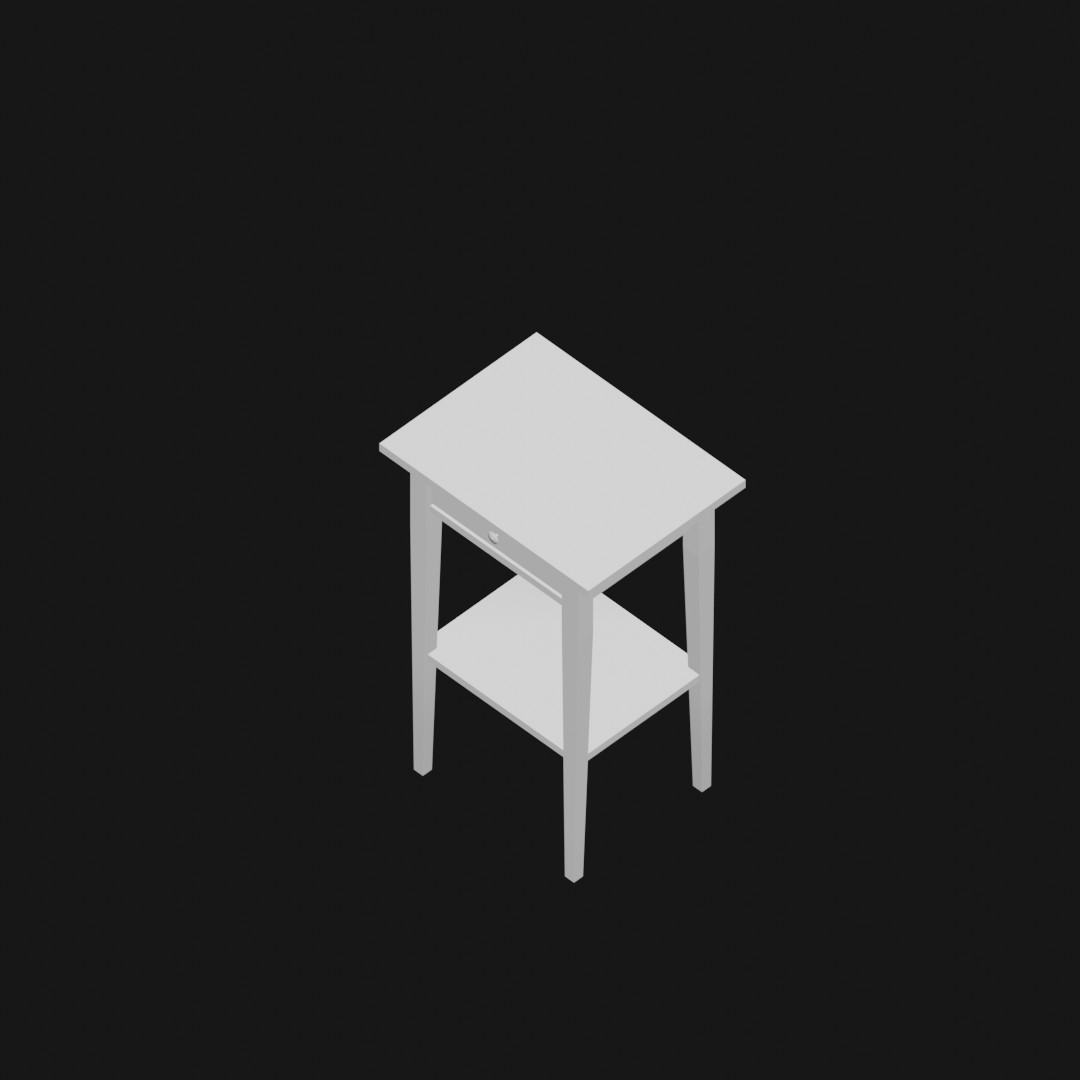
\includegraphics[width=\textwidth]{dissertation/images/assembledModel.jpg}
        \caption{The fully assembled bedside table.}
        \label{fig:syn1}
    \end{subfigure}
    ~ %add desired spacing between images, e. g. ~, \quad, \qquad, \hfill etc. 
      %(or a blank line to force the subfigure onto a new line)
    \begin{subfigure}[b]{0.45\textwidth}
        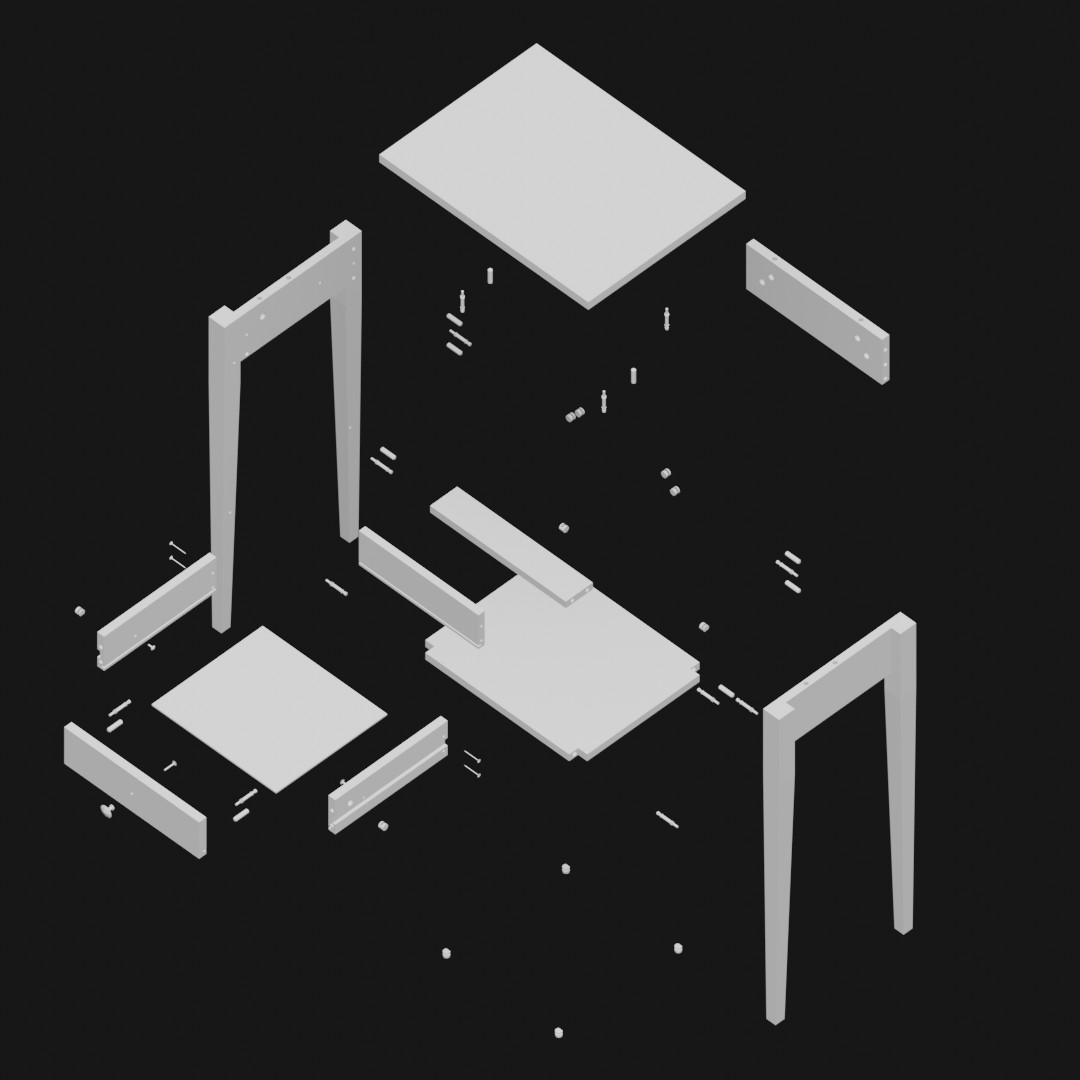
\includegraphics[width=\textwidth]{dissertation/images/explodedModel.jpg}
        \caption{An exploded view of the bedside table.}
        \label{fig:syn2}
    \end{subfigure}
    ~ %add desired spacing between images, e. g. ~, \quad, \qquad, \hfill etc. 
    %(or a blank line to force the subfigure onto a new line)    
    \caption{The fully assembled model of the IKEA HEMNES bedside table, including custom 3D models for each part, a view showing parts all in accurate locations and a view showing each individual part.}
    \label{fig:explode}
\end{figure}

% exploded view of 3D model

\section{Pilot Test}

After implementation was initially complete a pilot test was conducted which helped to highlight any issues with the system. One issue which became apparent during the pilot test was that the participant often was not sure if they had to screw in particular parts. Another issue was that if the location of a step was outside of the field of view of the participant, they would sometimes struggle to find the part to add. Lastly, when using the 'view' command, some parts did not appear large enough to be able to tell what they were.

Before conducting final tests, these issues were solved. To help inform users when to screw a part in, a text indicator was added that would send a message to the display when a part was to be screwed in. Since there is no text when a part is not to be screwed, the text appearing on particular steps should make it clear that the step is completed in a different manner. If more time was available before final testing, a better solution to this issue would be to animate arrows pointing in the rotation to screw a part on the spot where it should be added.

In order to solve the issue with parts being outside of the user's point of view, a small arrow was added to the viewport that points in the direction of where the part is to be added. When the part is not in the field of view the arrow is visible and pointing in its direction and when it enters the centre of the field of view, the arrow disappears. To implement this, first an image of an arrow was created. It is a tall transparent .png image with a small arrow at the top. This means that the image can be rotated around its centre point and appear as if the arrow is rotating around in a circle at the edge of the screen. The direction for the arrow to point on the screen was calculated using the code in listing \ref{lst:arrow}.

\begin{lstlisting}[language=c++, caption={The code for finding the direction of the arrow and showing/hiding the arrow if it is on or off the screen.}, label=lst:arrow]
    Vector3 viewportPos = Camera.main.WorldToViewportPoint(targetObject.transform.position);
                
    if (viewportPos.x >= 0.0f && viewportPos.x <= 1.0f && viewportPos.y >= 0.0f && viewportPos.y <= 1.0f) {
        arrowImg.color = new Color(1,1,1,0);
    } else {
        arrowImg.color = new Color(1,1,1,1);
    }

    var camPos = Camera.main.transform.InverseTransformPoint(targetObject.transform.position);

    // Calculate the angle in degrees
    float angle = -Mathf.Atan2(camPos.x, camPos.y) * Mathf.Rad2Deg;

    // Rotate the arrow to point towards the target
    arrow.transform.localEulerAngles = new Vector3(0,0, angle);

\end{lstlisting}

The world position of the part to be added is translated into a position relative to the viewport. This is then used to determine if the part is visible in the centre of the screen by checking the x and y coordinates of the relative position. The position of the part relative to the camera itself is then determined and the angle between these is calculated and converted to degrees. This angle is then set as the z rotation in the arrows local Euler angles.

To fix the issue with parts appearing too small in the view command, simple adjustments were made to the values within the implementation of the 'view' command to make the parts appear closer.

\section{Final Product}
% Include screenshots from runtime
% Talk about screw indicator as an incomplete feature compared to the design
The final product after implementation appeared as follows (note that the positioning and appearance of items on the recording of the Hololens display appears slightly different to how it appears in the user's perspective):

\begin{enumerate}
    \item The application starts and the user must choose between using animated instructions or object tracking instructions (If using object tracking, the user can also activate wide field of view).
    \item The user must then say "start" to initialise the instructions.
    \item The user is put on an initial step which contains no instruction and they must move on to the next step to progress.
    \item The step begins and the current part is highlighted in the correct location along with it's name appearing on the screen. Figure \ref{fig:initpos} shows the arrow which points to the correct location of the part if it is outside the user's field of view. For object tracking, the tracking object will appear in it's init position, ready to be tracked.

    \begin{figure}[hbt!]
        \centering
        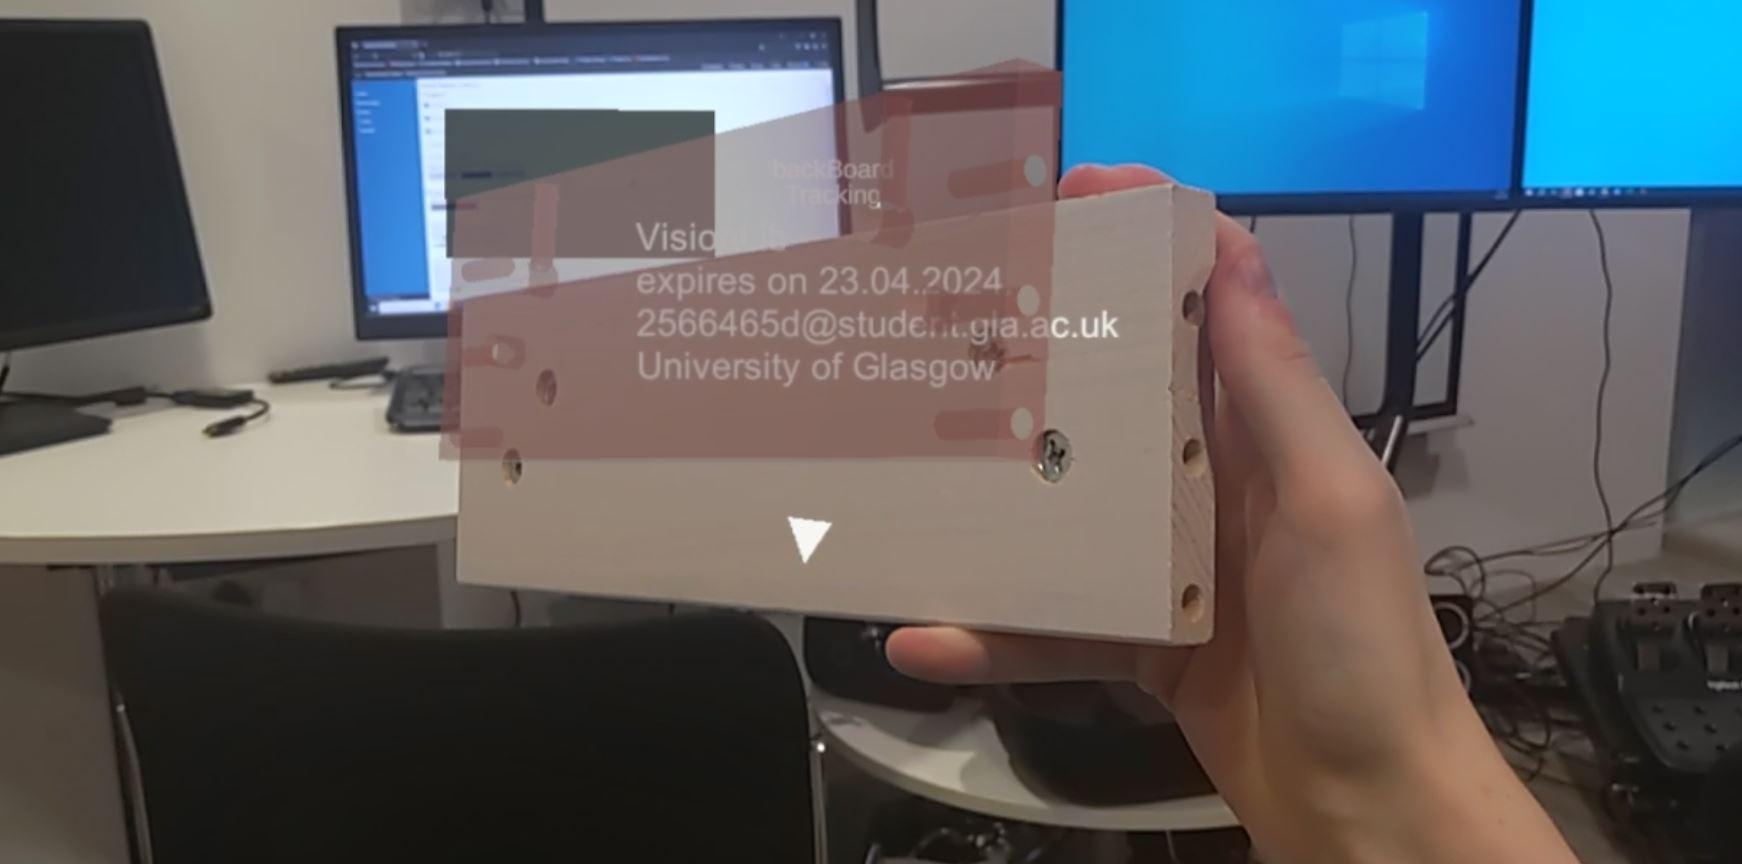
\includegraphics[width=0.7\linewidth]{dissertation//images/initPose.JPG}
        \caption{The tracking part in it's init position}
        \label{fig:initpos}
    \end{figure}

    \begin{figure}[hbt!]
        \centering
        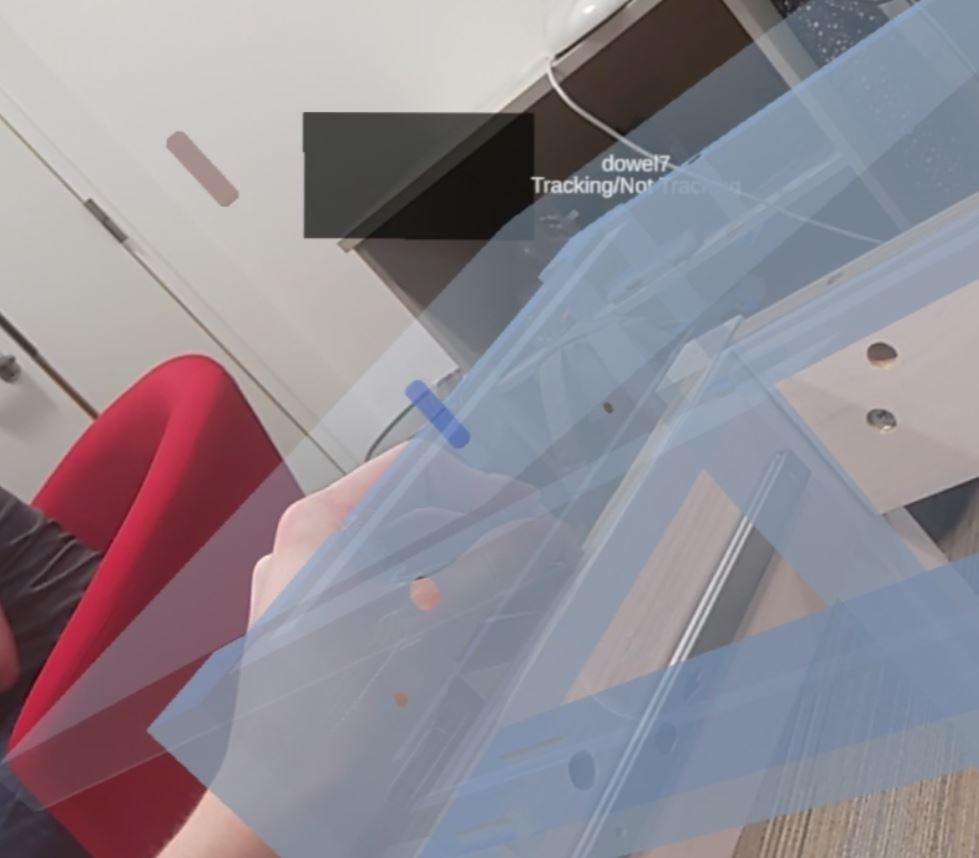
\includegraphics[width=0.5\linewidth]{dissertation//images/partWaiting.JPG}
        \caption{The current part (blue) highlighted in the correct location.}
        \label{fig:partWaiting}
    \end{figure}

    For animation, the animation object will start cycling it's animation.
    \item When the tracking/animation part reaches the correct position, it will appear green as shown in figure \ref{fig:correctPos}.

    \item The user then moves onto the next step and repeats until the process is complete.
    \item Once the last step is complete, a message is displayed to declare that the assembly is done (figure \ref{fig:complete}).

    
\end{enumerate}

\clearpage

\begin{figure}[hbt!]
    \centering
    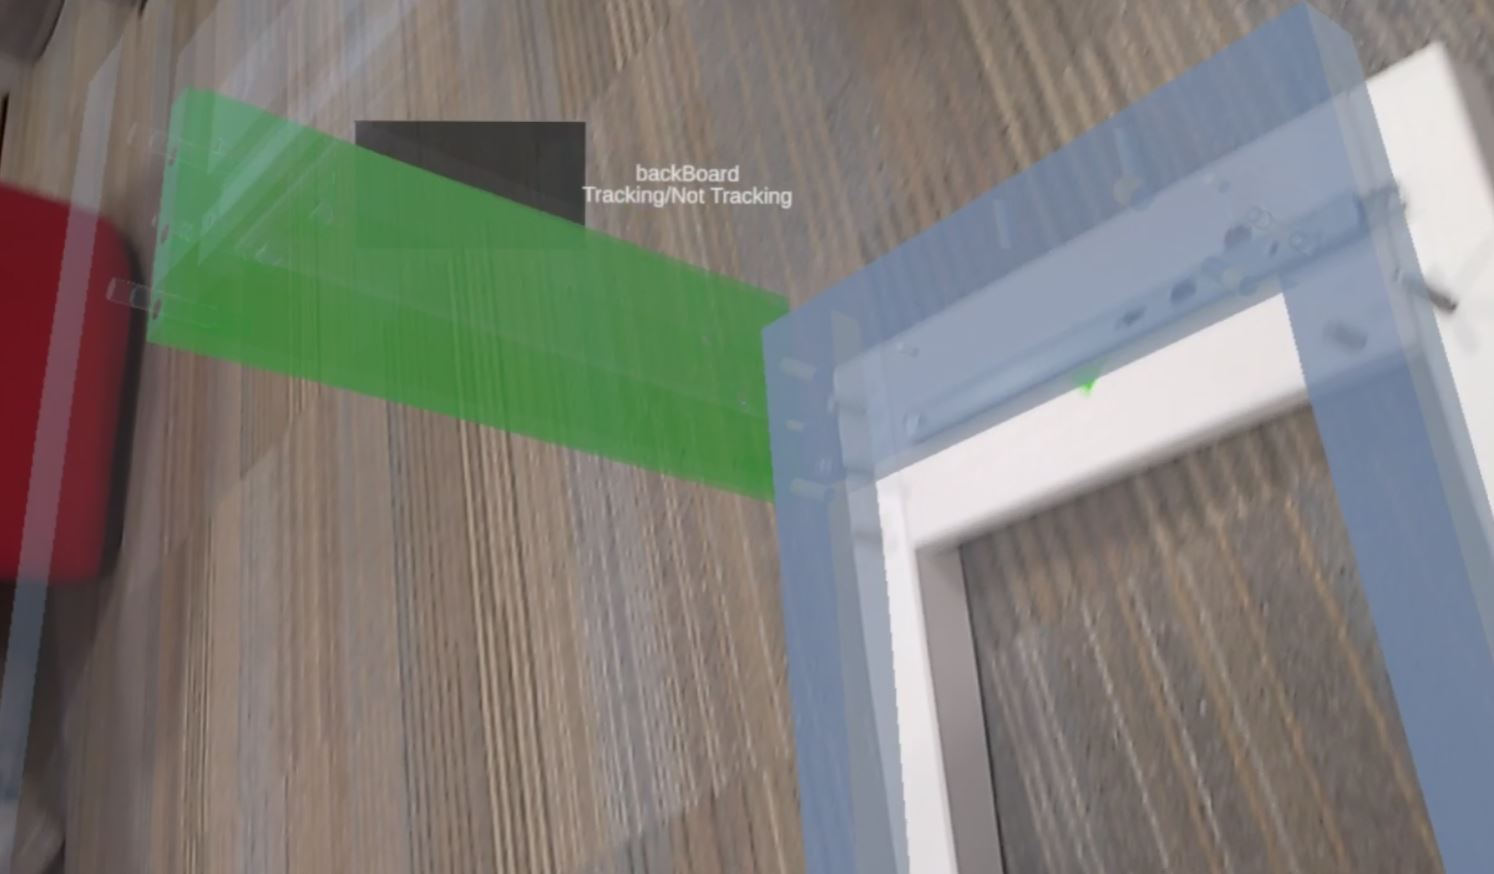
\includegraphics[width=0.7\linewidth]{dissertation//images/correctPos.JPG}
    \caption{The tracking/animation part in the correct location}
    \label{fig:correctPos}
\end{figure}

\begin{figure}[hbt!]
    \centering
    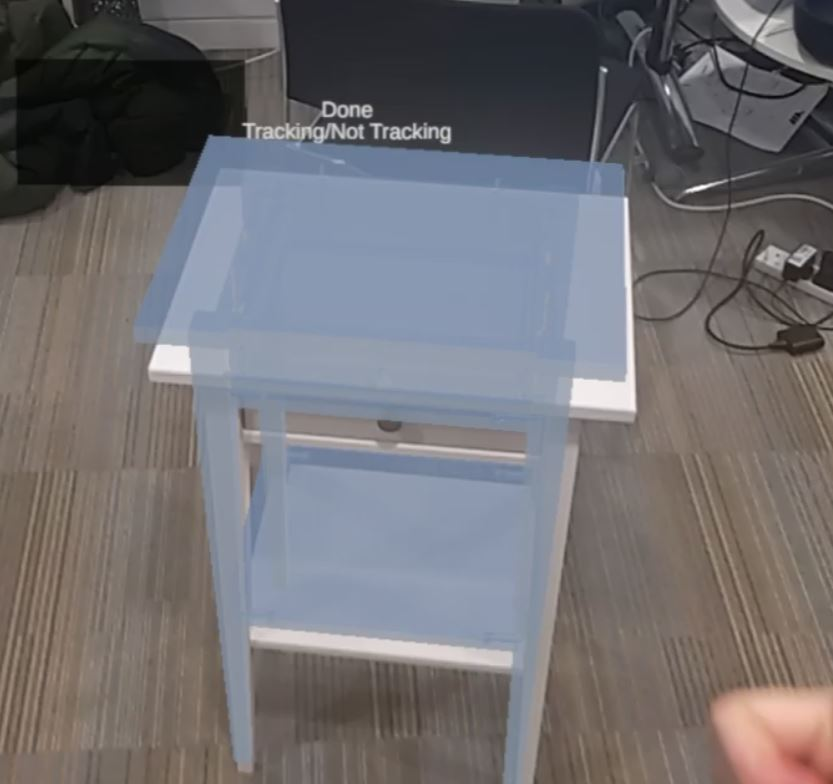
\includegraphics[width=0.5\linewidth]{dissertation//images/complete.JPG}
    \caption{The assembly in a finished state.}
    \label{fig:complete}
\end{figure}

\subsection{Issues}

\begin{itemize}
    \item The screw indicator did not match the way it was designed. This was due to time limitations.
    \item Tracking parts do not follow the users perspective and move strangely when the head tilts and moves. This was caused by issues with the camera offset from the ground.
    \item During particular steps which involve components, the full assembly appear wrong. This is because of the way the parent positions are set. Components cannot set their parent's position while their children parts are the active steps.
\end{itemize}

%==================================================================================================================================

\chapter{Experimental Design}
\label{chap:expdesign}

\section{Experiment Options}

There are a range of options when it comes to evaluating the effectiveness of a system. Potential users in this scenario would be assembling a piece of flatpack furniture with only a set of instructions and possibly another person to work with. Each user will have different skill levels when it comes to using tools and putting together pieces which means that assessing different types of instructions can be difficult. There are different aspects of the building process which can be measured such as assembly time, error rate or user approval rating. Measuring quantitative data alone was an option that was considered as if done well, would provide good data and allow for a strong analysis. However, it was deemed unsuitable for this case. Quantitative data such as time taken to assemble furniture would differ greatly between participants based on skill level and ability. This could cause mixed results across different types of instructions and would be useless data. Another option was to make each participant build a piece of furniture once with the paper instructions and once with the AR instructions. This was rejected as participants would be able to assemble the furniture quicker and easier after they already had done it once. In the end it was decided that a qualitative think aloud experiment in conjunction with recording error rates would result in the best findings. The data consists of strong user feedback and can be categorised to allow for effective evaluation. More specifically, the idea was for participants to speak aloud any time they felt confused or unsure what to do during the assembly process. These complaints could be categorised and and results could be compared across instruction types.

\section{Pilot Test}

While the idea for the experiment had been considered, it still had to be refined before it could be carried out. In order to see what worked best, a pilot test was conducted which followed the basic concept of a think aloud experiment with comments on particular moments of confusion or being unsure. The test was conducted using the animated instructions on the Hololens.

The pilot test highlighted issues with the format of the experiment. During the pilot test comments were noted but not categorised immediately. This resulted in too much time being spent on writing comments and difficulty in giving full attention to the ongoing assembly process. Another issue was that participants would sometimes hesitate to say if they were unsure, resulting in inaccurate results. Finally, the need for a good introductory script and tutorial on using the technology became clear as fundamental parts of the process were not being followed correctly, for example, the participant often forgot that they could use the 'view' command to get a closer look of the current part they were on.

\section{Final Experimental Design}

Based on the results of the pilot test, the experiment was adjusted. Participants were tasked with assembling a full piece of flatpack furniture with a provided set of instructions. 

\subsection{Furniture}

For this study the chosen piece of flatpack furniture was the IKEA HEMNES bedside table \citep{noauthor_hemnes_nodate}. This was chosen as it is a small piece of furniture that does not have too many parts but still has a certain amount of complexity to properly test the instructions. The table was assembled as shown in the paper instructions minus a few steps. The rails for the drawer were screwed on at the start, the feet were never added and the drawer was never screwed to the rails. These adjustments were made to avoid difficulty in disassembly between participants.

\begin{figure}[hbt!]
    \centering
    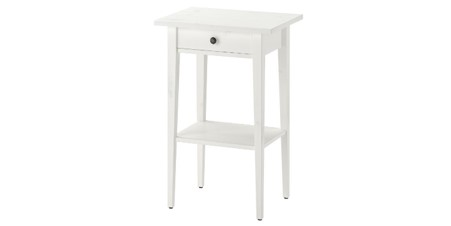
\includegraphics[width=0.7\linewidth]{dissertation//images/bedsideTable.jpg}
    \caption{The IKEA HEMNES bedside table \citep{noauthor_hemnes_nodate}}
    \label{fig:hemnes}
\end{figure}

\subsection{Measurements}

Participants were asked to think aloud as they were assembling the piece. Specifically they were asked to state if they found themselves in any moment of being unsure of confused. These comments were recorded with either a quote or a description of the issue. In the case that a participant was clearly and obviously unsure about what they were doing but never stated it, or they made a mistake without realising, this was also noted. Before the experiment, a group of categories were created that these issues could be sorted into:

\begin{itemize}
    \item \textbf{Part Identification}
    
    When the participant cannot find a part, initially selects a wrong part or is unsure which part to use. 
    
    \item \textbf{Location}
    
    When the participant is unsure about where to place the current part or initially places in the wrong spot.
    
    \item \textbf{Orientation}
    
    When a participant is unsure about what rotation a part should be placed in or initially places with the wrong rotation.
    
    \item \textbf{Progression}
    
    When a participant is unsure about what their next step requires them to do or if they move on to the wrong next step.

    \item \textbf{Tracking}

    This is only used during an experiment that uses object tracking. Whether or not the participant actually used the tracking and any other issues related to it.
    
    \item \textbf{Error}
    
    When a participant moves on to the next step while the previous step is still incorrect.
    
    \item \textbf{Other}
    
    Any other issue that does not fit a category or any other comment the participant makes.
    
\end{itemize}

Once the issues were categorised, they were given a severity score between 1 and 3. It was important that the distinction between these scores were made very clear to avoid bias in the rankings. Therefore each score level was given a clear definition. Issues which were small and insignificant to the overall progression were ranked one. Issues ranked with a two were issues that caused some delay but were not be detrimental to the ability to finish the assembly. Finally, issues ranked with a three were issues which would stop the assembly from being completable, these issues required assistance to be given to the participants to get them back on track.

\subsection{Procedure}

At the start of the experiment the introduction script is read to the participant along with a brief introduction of the Hololens and how to use the application if they will be using it. The application is a prototype and does not put a strong focus on the user interface or a tutorial. This means that a user introduction is required to not allow difficulty in understanding the application or hardware to get in the way of evaluating the effectiveness of the instructions method.

A short survey was conducted after the introduction of the experiment to get an initial understanding of the experience and variety of the participant group.

A group of nine participants were selected for the experiment. The group had a four to five female-male split and covered an age range of 20-25. The members of the group had varied experience in using AR technologies. A few had used simple AR applications on smartphones while others had used VR headsets. Only one had used a head mounted display previously. There was also a variance in their confidence with building flatpack furniture. Every participant said they had previously assembled flatpack furniture. The average confidence level for an assembly task was 3.33 out of 5. All but one participants said they had previously felt confused by paper instructions.

Participants were equally split into three different groups, one control group and two experimental groups. The control group were asked to assemble the bedside table using only the paper instructions. The first experimental group used the Hololens instructions without any object tracking. This entailed assembling the bedside table exclusively using the part animations to show where parts should be added. The last experimental group used the Hololens instructions with a mix of animated parts and tracked parts. This meant that while some parts of the assembly were animated, others were tracked to help confirm the positioning of a part.

During the experiment, any time the participant reached a moment of being unsure or confused, it was noted into this table, \ref{tab:blankissues} with a brief description, at the correct step. A category was selected in the moment but experiments were recorded and viewed later to confirm that issues were noted correctly.
    \begin{table}[!ht]
         \caption{
         Blank template for recording issues from participants
         }\label{tab:blankissues}
        \centering
        \rowcolors{2}{}{gray!3}
        \begin{tabular}{@{}l|llllll@{}}
            \textbf{Part} & \textbf{Part Identification} & \textbf{Location} & \textbf{Orientation} & \textbf{Progression}  & \textbf{Error} & \textbf{Other} \\ \hline
            \textbf{1}  & ~ & ~ & ~ & ~ & ~ & ~ \\ 
            \textbf{2}  & ~ & ~ & ~ & ~ & ~ & ~ \\ 
            \textbf{3}  & ~ & ~ & ~ & ~ & ~ & ~ \\ 
            \textbf{.}  & ~ & ~ & ~ & ~ & ~ & ~ \\ 
            \textbf{.}  & ~ & ~ & ~ & ~ & ~ & ~ \\ 
            \textbf{.}  & ~ & ~ & ~ & ~ & ~ & ~ \\ 
        \end{tabular}
    \end{table}

After this section of the experiment was completed, participants that used the Hololens instructions were asked to complete a survey about their experience. This survey was mainly used as a backup source to the results on the issues table. It helped to identify and confirm themes that arose in the experiment. The questions on the survey were as follows:

\begin{itemize}
    \item \textbf{How easy did you find assembling the furniture with the given instructions?}
    
    \centerline{(Difficult) 1 2 3 4 5 (Easy)}
    
    \item \textbf{How enjoyable did you find assembling the furniture with the given instructions?}

    \centerline{(Not Enjoyable) 1 2 3 4 5 (Very Enjoyable)}

    \item \textbf{How useful did you find the arrow that points towards the next step?}

    \centerline{(Not useful) 1 2 3 4 5 (Very useful)}

    \item \textbf{How clear did you find where to place the next step?}

    \centerline{(Not Clear) 1 2 3 4 5 (Very clear)}

    \item \textbf{How sure were you on if a part was to be screwed in or not?}

    \centerline{(Not sure) 1 2 3 4 5 (Very sure)}

    \item \textbf{How useful did you find having a guide on where to place the assembly so far while adding the current step?}

    \centerline{(Not useful) 1 2 3 4 5 (Very useful)}

    \item \textbf{Any other comments about your experience using these instructions?}
\end{itemize}

%==================================================================================================================================
\chapter{Evaluation} 
\label{chap:evaluation}

The aim of this experiment was to prove that using augmented reality instructions for assembling flatpack furniture will lead to an improved experience for users over paper instructions. It sought out to find the benefits of using AR instructions in flatpack furniture assembly.

\section{Results}

The experiment was successfully conducted by all 9 participants. All participants of the paper and animation group were able to successfully complete the bedside table using the given set of instructions. Participants that used the tracking instructions all stopped using the tracking functionality at some point and completed the furniture without it. Results were recorded for the control group and two experimental groups. Each participant was given a score based on the issues they had and the severity of the issues. These scores are highlighted in table \ref{tab:issueScores}.

% Define command for coloring cells based on their values
\newcommand{\coloredcell}[1]{%
    % Calculate the mix ratio based on the value
    \pgfmathsetmacro{\mixratio}{100*(#1-19)/(77-19)}
    % Round the mix ratio to an integer
    \pgfmathtruncatemacro{\mixratio}{\mixratio}
    % Calculate complementary ratio
    \pgfmathsetmacro{\compratio}{100-\mixratio}
    % Set the cell color using the mix ratio
    \cellcolor{red!#1!white}{#1}
}

\begin{table}[h]
\caption{
         The total issue scores for each participant in each category and altogether
         }\label{tab:issueScores}
\centering
\begin{tabular}{|l|l|p{0.5cm}|l|l|l|l|l|}
\hline
Participant & Instructions & Part ID & Location & Orientation & Progression & Error & Total \\ \hline
1           & Animation    & 2                   & 0        & 6           & 3           & 8     & \coloredcell{19}    \\ \hline
2           & Paper        & 9                   & 14       & 11          & 12          & 31    & \coloredcell{77}    \\ \hline
3           & Animation    & 8                   & 5        & 9           & 4           & 10    & \coloredcell{36}    \\ \hline
4           & Animation    & 12                  & 3        & 7           & 7           & 6     & \coloredcell{35}    \\ \hline
5           & Paper        & 2                   & 15       & 11          & 2           & 12    & \coloredcell{42}    \\ \hline
6           & Tracking     & 6                   & 12       & 3           & 4           & 6     & \coloredcell{31}    \\ \hline
7           & Paper        & 10                  & 8        & 7           & 3           & 12    & \coloredcell{40}    \\ \hline
8           & Tracking     & 8                   & 7        & 3           & 3           & 7     & \coloredcell{28}    \\ \hline
9           & Tracking     & 8                   & 5        & 10          & 4           & 3     & \coloredcell{30}    \\ \hline
\end{tabular}
\end{table}

The table highlights the range in different scores per participant. Across all forms of instructions there was at least some difficulty in assembling the furniture. The lowest score for error was 3 which is equal to one error that required assistance to fix before progressing further. The highest error score was 31. Such a range in values suggests a large variability in the participants accuracy in assembling the furniture. Grouping these values by category highlights the level of difficulty had by participants using each instruction type. This is shown in figure \ref{fig:avgScores} which shows the average total score for participants in each category. \clearpage

\begin{figure}[hbt!]
    \centering
    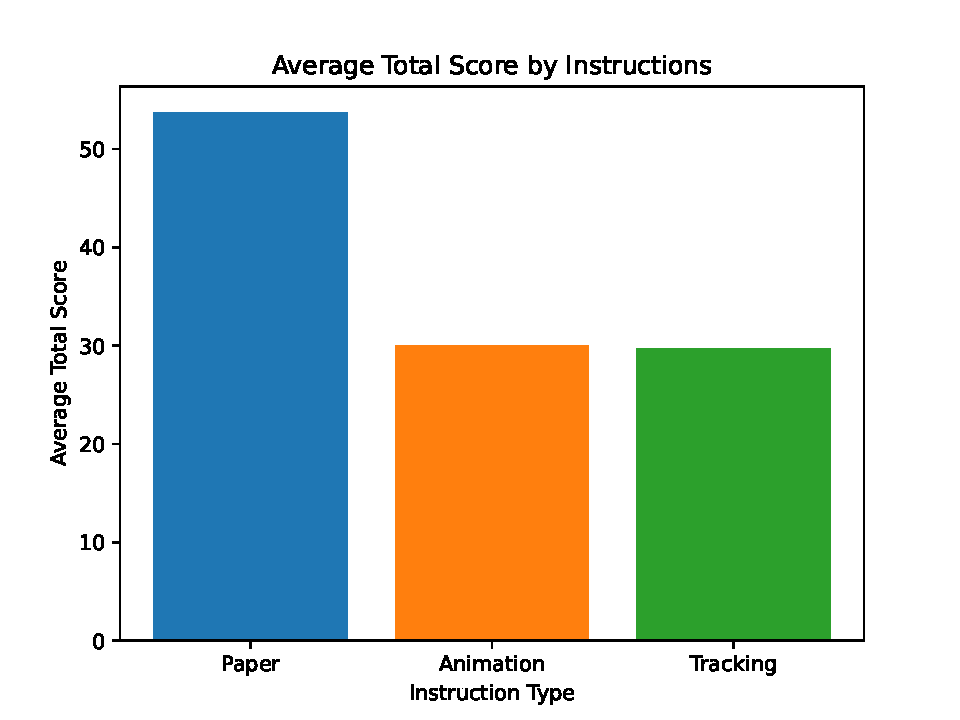
\includegraphics[width=0.75\linewidth]{dissertation//images/avgScores.pdf}
    \caption{The average total issue scores per category of instructions.}
    \label{fig:avgScores}
\end{figure}

On average, participants using the paper instructions had more difficulty and made more mistakes than both the other groups. While this demonstrates that the difficulty levels were higher for paper instructions than any augmented reality instructions, it is important to evaluate where participants had trouble and what may have caused it. Figure \ref{fig:stepScores} shows where in the assembly process participants had the most trouble.

% add average score per issue type

\begin{figure}[hbt!]
    \centering
    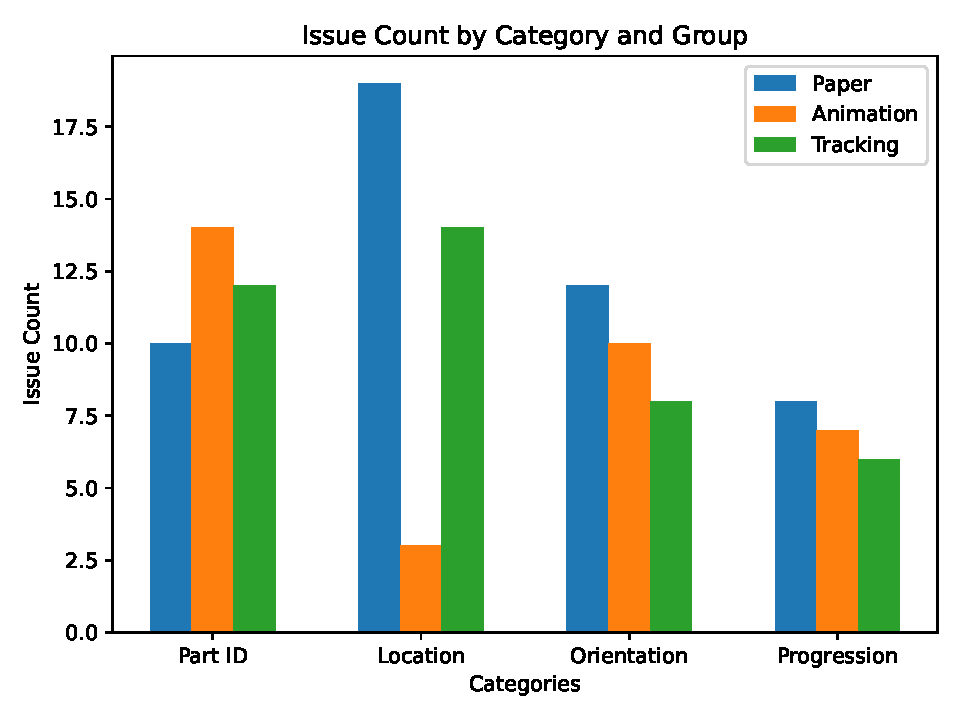
\includegraphics[width=0.75\linewidth]{dissertation//images/issuesPerCategory.pdf}
    \caption{The total number of issues had in each category by group.}
    \label{fig:issuesPerCategory}
\end{figure}

Figure \ref{fig:issuesPerCategory} shows the total number of issues each group had in each category. Participants had the least trouble telling which part to use with paper instructions. However, they had the most trouble telling which location to place them in. The animation instructions proved to be very effective at telling participants the location. The tracking count for location is particularly high compared to animation. Paper suffered the worst from orientation issues but none of the scores were very far from each other. The same can be said for progression issues. Paper's worst performance was with location and their best was in progression. Animation's worst performance was in part identification and their best was in location. Tracking's worst performance was in location and their best was in progression.

\begin{figure}[hbt!]
    \centering
    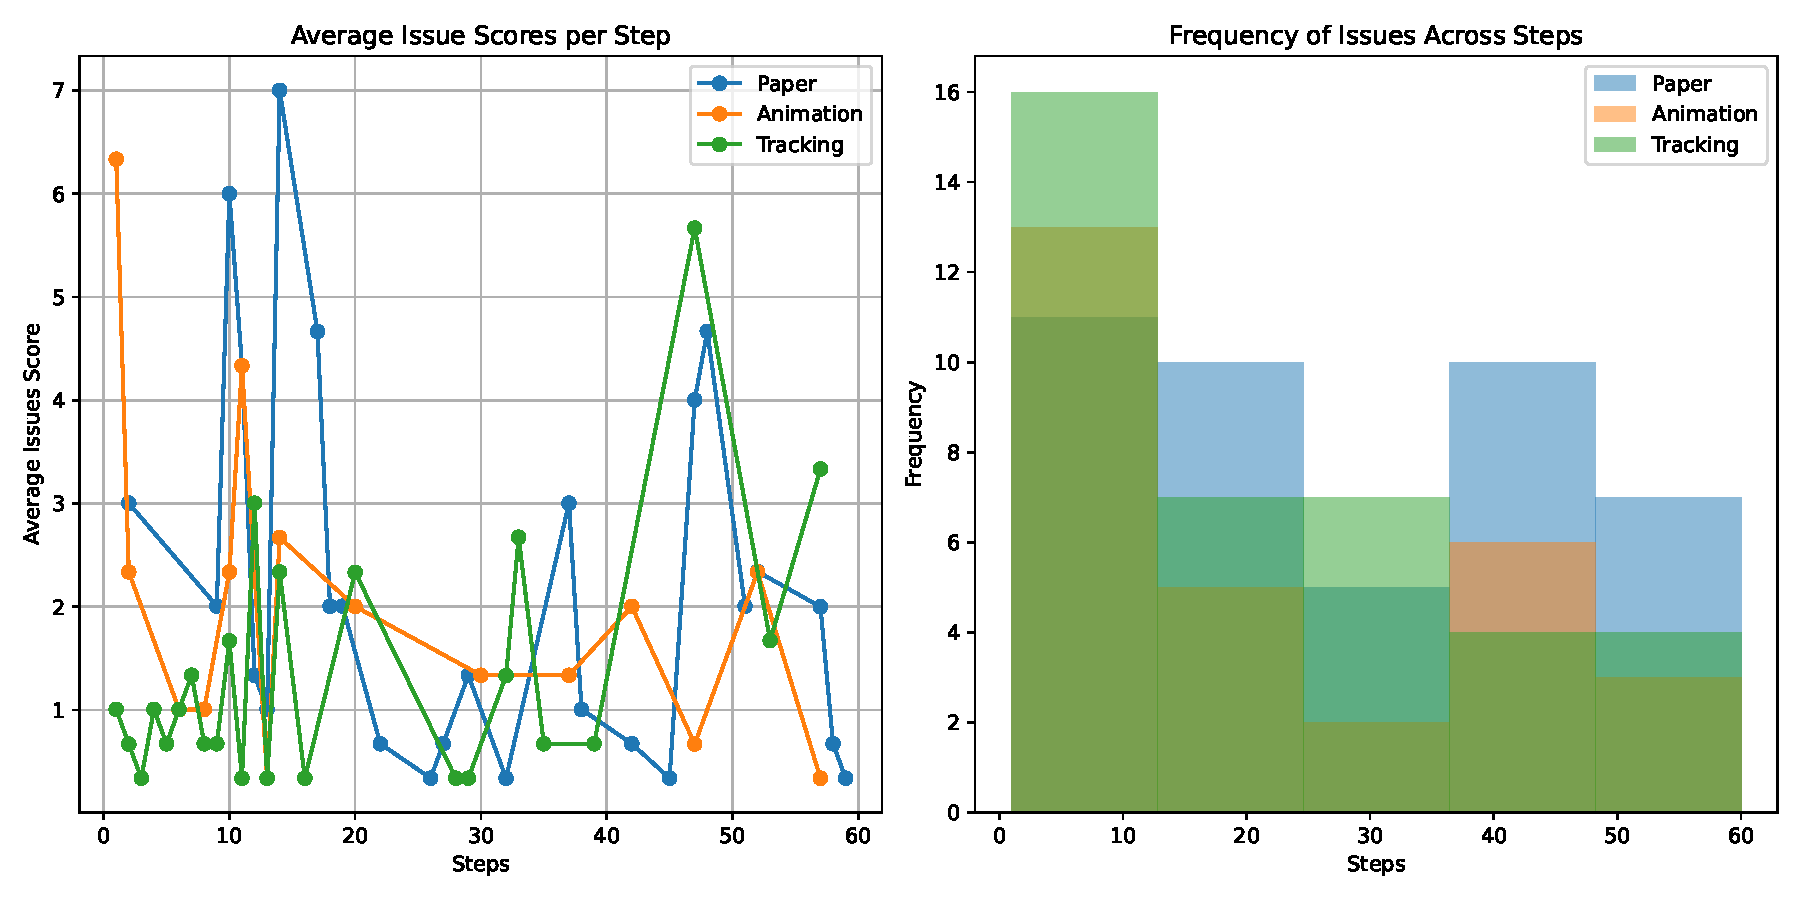
\includegraphics[width=0.9\linewidth]{dissertation//images/scoresPerStep.pdf}
    \caption{One the left, the average issue score per step for each category (Values of 0 have been removed). On the right, the frequency of issues occurring at each step, grouped into 5 bins, per category. These are not affected by the value of the score at these points, rather the number of times the score is not 0 and how many participants had this issue.}
    \label{fig:stepScores}
\end{figure}

The steps participants from each group had the most trouble with are highlighted using both charts. The line chart highlights steps which caused the most significant issues while the histogram shows how commonly there were issues throughout the assembly. Spikes in the line chart could represent a particularly difficult step for that specific set of instructions. For example, the tallest blue (paper) spike represents a step which involves placing a shelf on the middle of the first set of legs. This is a step which involves selecting the correct part and placing it in the correct orientation. The part has 4 holes one one side and none on the other. Many participants had difficulty selecting the correct way round to place this part which led to spikes in issue scores at this point. However, it is clear that this step was more difficult for people using paper instructions than those using the AR instructions as the blue spike is much greater than the other spikes. The histogram also shows that the frequency of issues was high around this point in the assembly for paper instructions which also highlights the fact that many participants had this issue. One problem with the line chart alone is that it can strongly be affected by individual outliers. The last green (tracking) spike represents the step of adding a screw to the drawer for attaching the handle to. Most of the tracking participants only had a very small issue with this step with 2 out of 3 having a score of 1, whereas 1 participant had a score of 8 which creates a spike in the chart that is not particularly representative of the entire group. The histogram has no high values at this point for tracking users which suggests that there was not much difficulty from all tracking users around this step.

Looking at the histogram in figure \ref{tab:issueScores} shows a theme for each of the instruction types. Both animation and tracking instructions start very high with a large amount of issues happening between participants followed by the frequency quickly lowering as the steps progress. On the other hand, the paper instructions start lower than the other two but after this it remains mostly higher than the other types for the rest of the steps. This could be explained by the learning curve of trying to use the augmented reality instructions on the Hololens. According to the survey taken at the start of the experiment, all of the participants had assembled furniture using paper instructions before whereas very few had used a Hololens and none had used any of the newly designed instructions. It would make sense that participants using the AR instructions for the first time would have difficulty understanding and getting used to it at the start. 

While this data in a quantitative form can be useful, with the size of experimental groups used in this experiment, analysing the data like this is at risk of being affected by individual performances too much. It is important to evaluate the qualitative feedback given by the participants to identify themes and patterns. Doing this will help to backup the trends shown in the chart data.

\subsection{Paper Instructions Analysis}

Starting with the paper instructions, one issue participants had involved a step which required placing a group of tighteners to connect the second set of legs to the rest of the assembly. All 3 participants in the paper instructions group had some issue with one of the tighteners at this step shown in figure \ref{fig:paper7}.

\begin{figure}[hbt!]
    \centering
    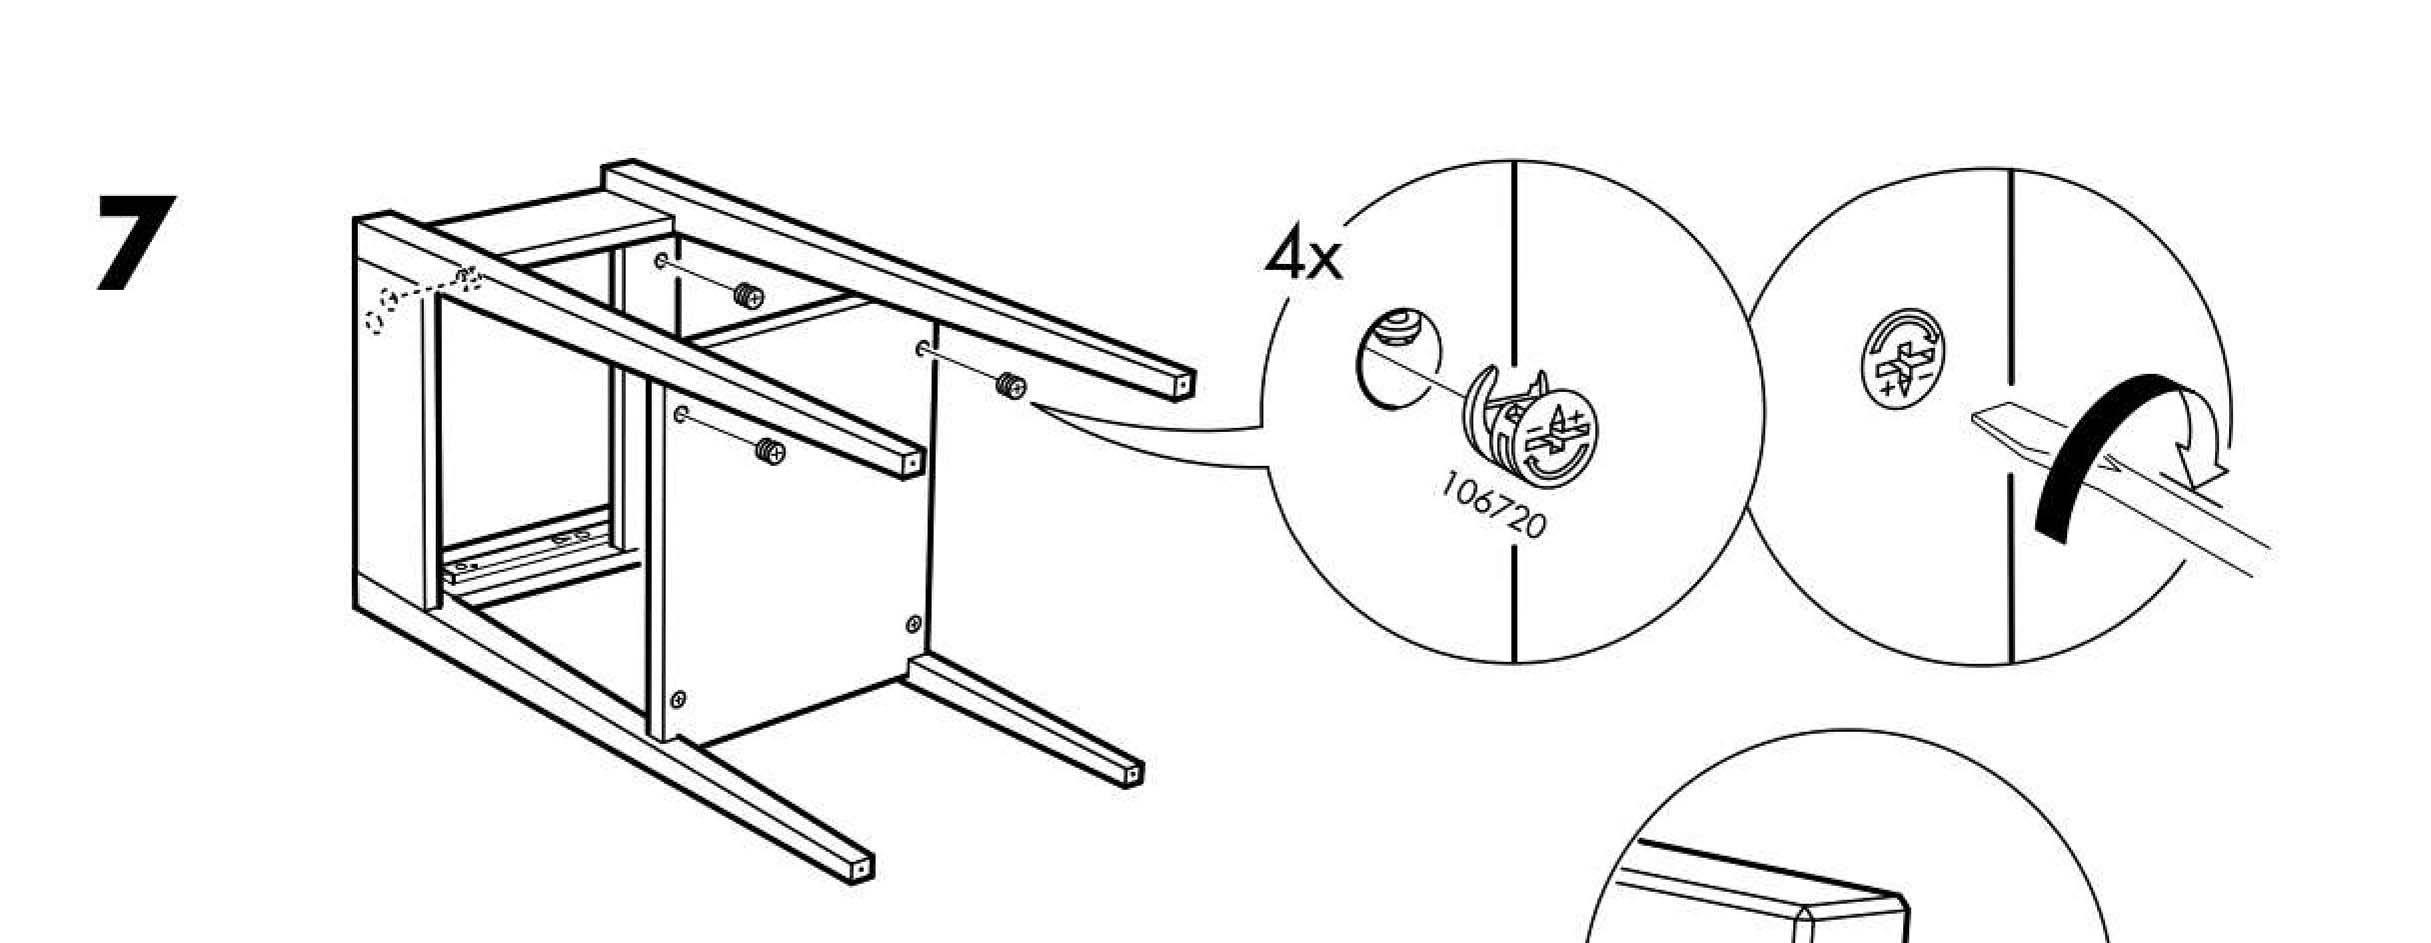
\includegraphics[width=0.75\linewidth]{dissertation//images/instructionsStep7.jpg}
    \caption{Step 7 of the Paper Instructions \cite{noauthor_hemnes_nodate}}
    \label{fig:paper7}
\end{figure}

The image shows that participants must screw in four tighteners in different spots of the assembly. The part that caused trouble for participants is the tightener which is obscured in the image. Two of the three participants had difficulty in finding which hole the instructions required them to place it in whereas the third participant could not even identify the fourth tightener on the instructions. This participant requested help to progress at this point. 

A very similar issue occurred earlier in the paper instructions. While it did not cause as much difficulty in progression as the issue in figure \ref{fig:paper7}, it was still notable for being the same in nature as it. Step 4 of the paper instructions required participants to place tighteners into parts connecting to the first set of legs. One of these tighteners was obscured in the same way as the tightener in figure \ref{fig:paper7}. One participant was unsure about which hole to place it in but made the correct decision eventually. Another participant required help to identify the correct spot. Uniquely, the last participant was not confident in their part selection due to 'misleading symbols on image of the part'.

% Backboard and drawer sides for orientation (also could mention under drawer connector)

Another issue participants had while using paper instructions was during a step which required adding a larger part to the assembly. The step involved placing two flat pieces onto the first set of legs. The pieces had holes on one face and not the other along with holes on each side which meant that it had to be placed in the correct orientation. The step shown in figure \ref{fig:paper3} caused trouble for all participants using the paper instructions.

\begin{figure}[hbt!]
    \centering
    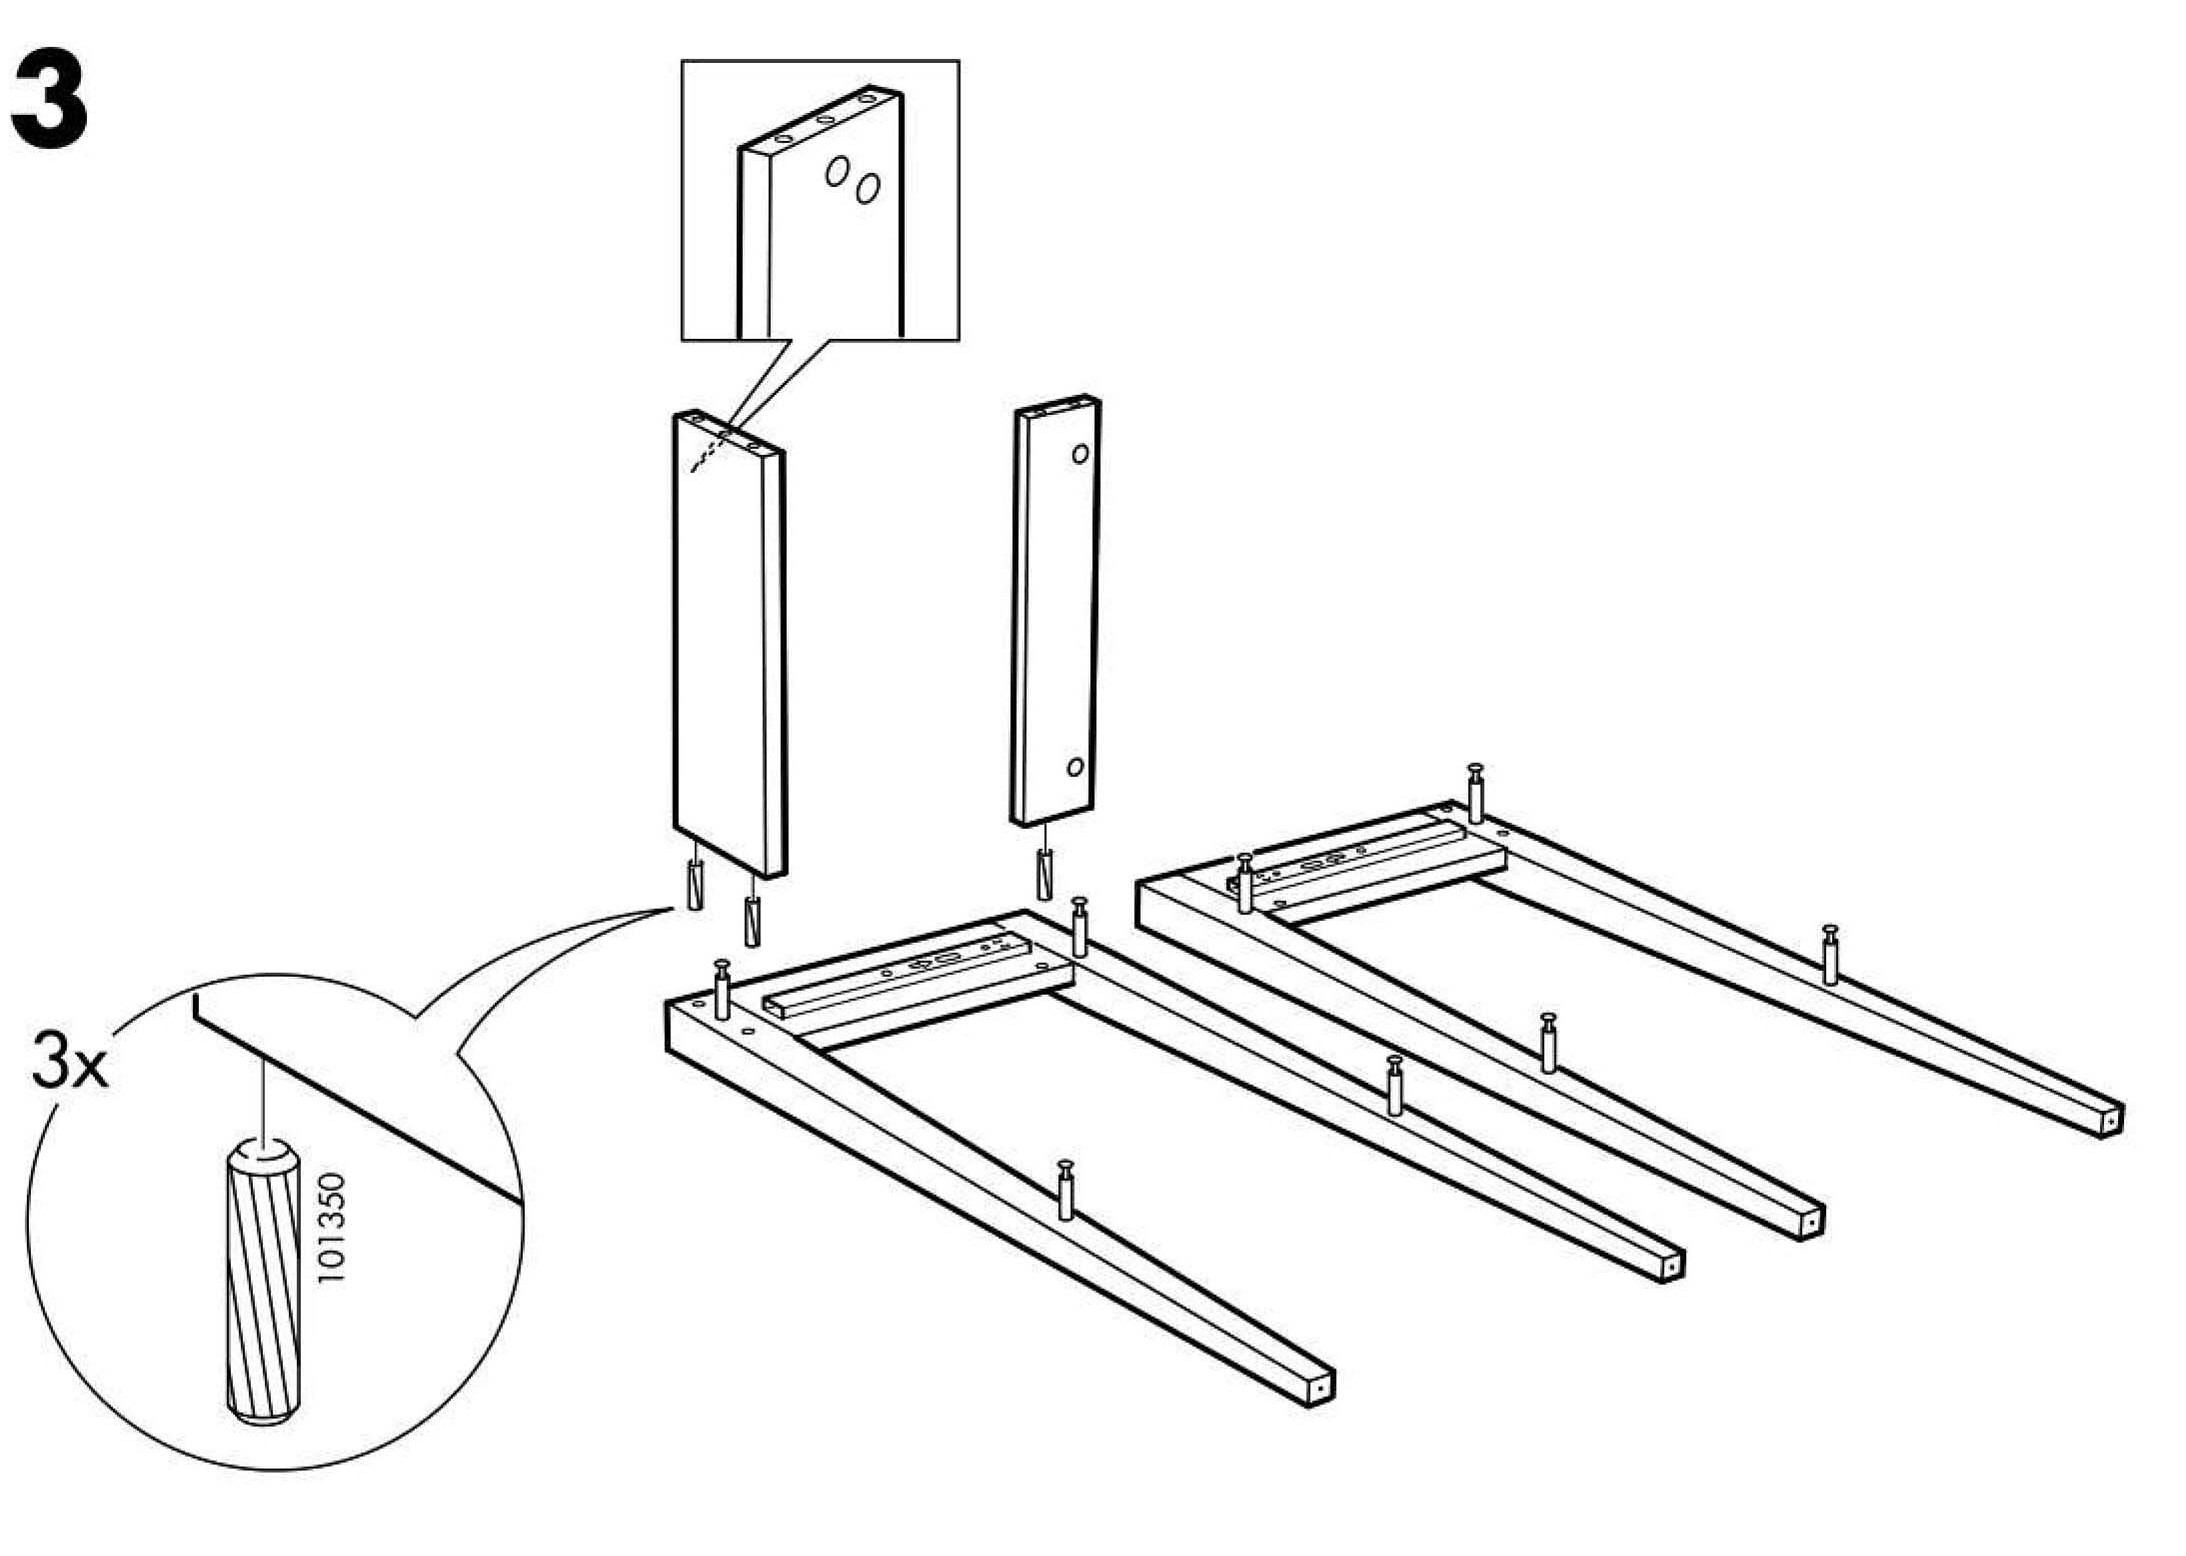
\includegraphics[width=0.6\linewidth]{dissertation//images/instructionsStep3.jpg}
    \caption{Step 3 of the Paper Instructions \cite{noauthor_hemnes_nodate}}
    \label{fig:paper3}
\end{figure}

The back board piece caused the most difficulty among the participants. The holes on this part face away on the image in the instructions. This meant that it could be placed in a way that looked correct as the holes faced away with the holes on the side being in the wrong place. Two out of the three participants placed it the wrong way around at least once before getting it right, with only one participant getting it right the first time after some confusion. The other part in this step also caused difficulty with two out of the three participants being unsure about the orientation it should be placed in. The last participant had a different issue at this point as they thought that this piece was meant to be the same as the back board piece which led to them selecting the wrong part.

Participants had similar difficulties later in the process when assembling the drawer component. The drawer has two side pieces which need to be attached to the front face of the drawer. These pieces have particular holes and grooves on each side which need to be placed the correct way. All paper participants had some form of difficulty with this step. One participant was unsure about their part selection when adding the first side part. Another participant was unsure about the orientation to place the first part in and initially placed it wrong before realising their mistake. The last participant placed both parts in the wrong orientation before being advised of their mistake.

% Write some positivity
Despite this, paper instructions had the lowest overall amount of issues with part identification. This shows that images of the parts can be very useful in identifying them compared to representation in 3D space. 

\subsection{Animation Instructions Analysis}

Participants using the animation variation of the augmented reality instructions faced issues across different steps of the assembly process. One issue involved the last step involving the first set of legs. These legs are an example of a component which is a part that is assembled out of other parts separately from the rest of the furniture and then added after. Since this is the first component, once it is fully assembled, there is a step which requires the participant to place the legs down in a new position. This confused two of the three animation participants. One participant said they could not tell when the step was complete and the other thought that they had to add the other legs piece at this point.

Another problem participants in the animated instructions faced involved starting the second set of legs. This step is the beginning of a new component which means that the next part is added separately from the assembly at that moment in time. When this happens the assembly gets put in a default position as shown in figure \ref{fig:anim20} which is different to the position it was in before.

\begin{figure}[hbt!]
    \centering
    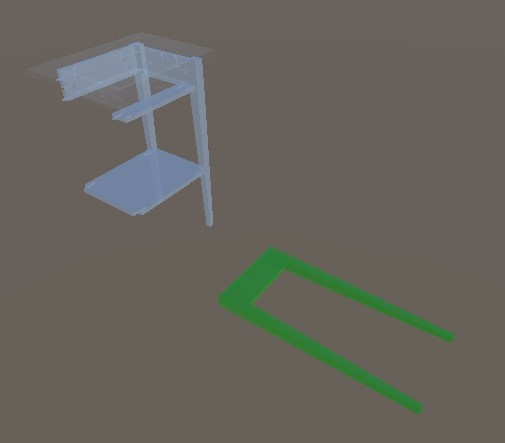
\includegraphics[width=0.5\linewidth]{dissertation//images/animationLegsLeft.jpg}
    \caption{Step 20 of the animation instructions}
    \label{fig:anim20}
\end{figure}

The part to be added (shown in green) is to be placed on the ground, however the rest of the assembly is placed in a new position which is irrelevant to the progress of the instructions. Since the last steps involve the main section of the furniture, participants were susceptible to getting confused by this step. Two of the participants expressed some form of trouble at this point. One said that it was unclear that the main assembly should be moved out the way at this point. The other said that the furniture appearing vertical with only one set of legs attached confused them.

\begin{figure}[hbt!]
    \centering
    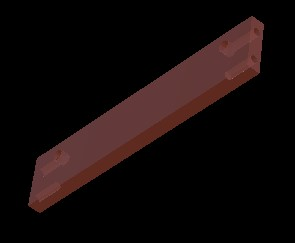
\includegraphics[width=0.4\linewidth]{dissertation//images/animationConnector.jpg}
    \caption{Step 11 of the animation instructions, as shown from the 'view' command}
    \label{fig:anim11}
\end{figure}

Participants had trouble during the step which required them to place a part that connects the two sets of legs at the front. The part is a long, flat piece with two holes on the top and holes in the side as shown in figure \ref{fig:anim11}. One participant had a lot of trouble with this step. They struggled to identify the correct part for a while until they required help to select it. The participant did try to use the 'view' command but they thought the part from this perspective appeared too far away.

The two other participants also had some difficulty at this stage however they both chose correctly after using the view command.

\begin{figure}[hbt!]
    \centering
    \begin{subfigure}[b]{0.45\textwidth}
        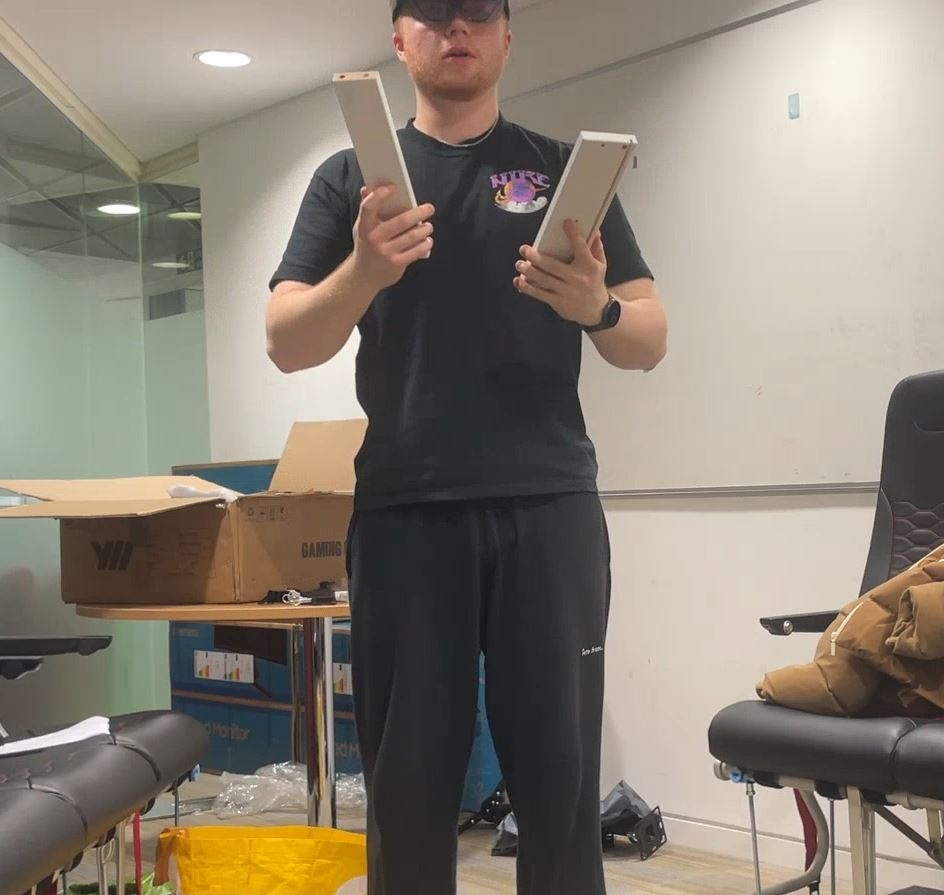
\includegraphics[width=\textwidth]{dissertation/images/expView.JPG}
        \caption{Participant using the view command to select between two parts.}
        \label{fig:expView}
    \end{subfigure}
    ~ %add desired spacing between images, e. g. ~, \quad, \qquad, \hfill etc. 
      %(or a blank line to force the subfigure onto a new line)
    \begin{subfigure}[b]{0.45\textwidth}
        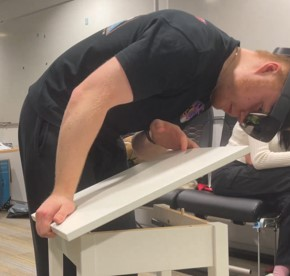
\includegraphics[width=\textwidth]{dissertation/images/expTop.JPG}
        \caption{Participant placing the top surface on while having trouble finding the correct orientation of the part.}
        \label{fig:expTop}
    \end{subfigure}
    ~ %add desired spacing between images, e. g. ~, \quad, \qquad, \hfill etc. 
    %(or a blank line to force the subfigure onto a new line)    
    \caption{A participant using the animation instructions experiencing the two most common issues in the animation group.}
    \label{fig:expAnim}
\end{figure}

A common issue across multiple steps of the process was confusion with the orientation of parts. The first step of the instructions involved choosing the first set of legs and placing them down correctly. One participant was unsure about the rotation and the other two placed the legs incorrectly with the flat face down at first.

Part identification and orientation issues were the most common for participants throughout the process. Difficulty with orientation led to seven errors overall whereas part identification only led to two errors. Examples of these issue are shown in \ref{fig:expAnim}

Some other comments of note were recorded during the animation instructions. One participant pointed out during a step which involved adding a very small part that they were struggling to see that part animating. A participant encountered an error that required help to fix as they accidentally skipped a step when they failed to notice the new step had started. On the other hand, another commented that using the instructions was 'quite good fun'. One participant said that the name of the part on the screen was very useful to identifying the correct part.

\subsection{Tracking Instructions Analysis}

The unique aspect of the tracking variation of the instructions was that it offered the ability to track parts in real space and then communicate to the user when the part was in the correct position. Participants generally tried to use this feature at the start of the instructions but all but one gave up at some point.

The reason for this is that tracking was very difficult to use in the context of the experiment. In the survey, one participant said that, "tracking had to be forced into position rather than being a guide on position." The tracking part would regularly lose tracking and be left behind. Sometimes it would latch onto other items in the room. On some occasions the tracking part would move away from the participant and end up in an unreachable location.

One participant tried to use tracking until step 14 at which point they gave up. They only used tracking to highlight the part in the correct location for one step. Another participant attempted to use tracking until step 10 and got the correct location from it for two steps. The other participant tried to use tracking all the way to the end but only successfully used it on three steps. When a participant uses the tracking instructions without utilising the tracking aspect, they are essentially using the animation instructions without the animation to guide them on the correct position or the 'view' command.

A reoccurring issue across the tracking instructions was finding the correct location for parts. Every participant had multiple steps in which they could not find a location. Participants commented that at a distance, the part showing the correct location would disappear, this is likely a unique bug to the tracking instructions. Overall, there were 14 issues involving part location across all of the tracking group. Each of these issues involved small parts like screws and dowels. 

Another issue that occurred multiple times throughout the tracking instructions was identifying the correct part. This was very high in comparison to the animation instructions, it was the only category in which they did not follow a similar level of issues. Each participant had multiple moments of difficulty involving finding the correct part. These issues involved both smaller and larger parts. There were 12 part identification issues in total across all the tracking participants. Two participants said that the name of the part being on the screen was a useful solution to this issue.

The next most common issue in the tracking instructions involved finding the correct orientation for parts. Each participant had at least one issue with orientation. This happened mostly on larger parts. There were eight orientation issues in total.

Two participants commented that it was not obvious enough when they had to screw a part in.

% Discussion about survey results
\subsection{Survey Feedback}

The main aim of the survey was to gain feedback from the experimental groups to confirm if it is similar to the results from the issues recorded during the experiment. The results mostly matched what was expected but a few interesting points were highlighted.

\begin{figure}[hbt!]
    \centering
    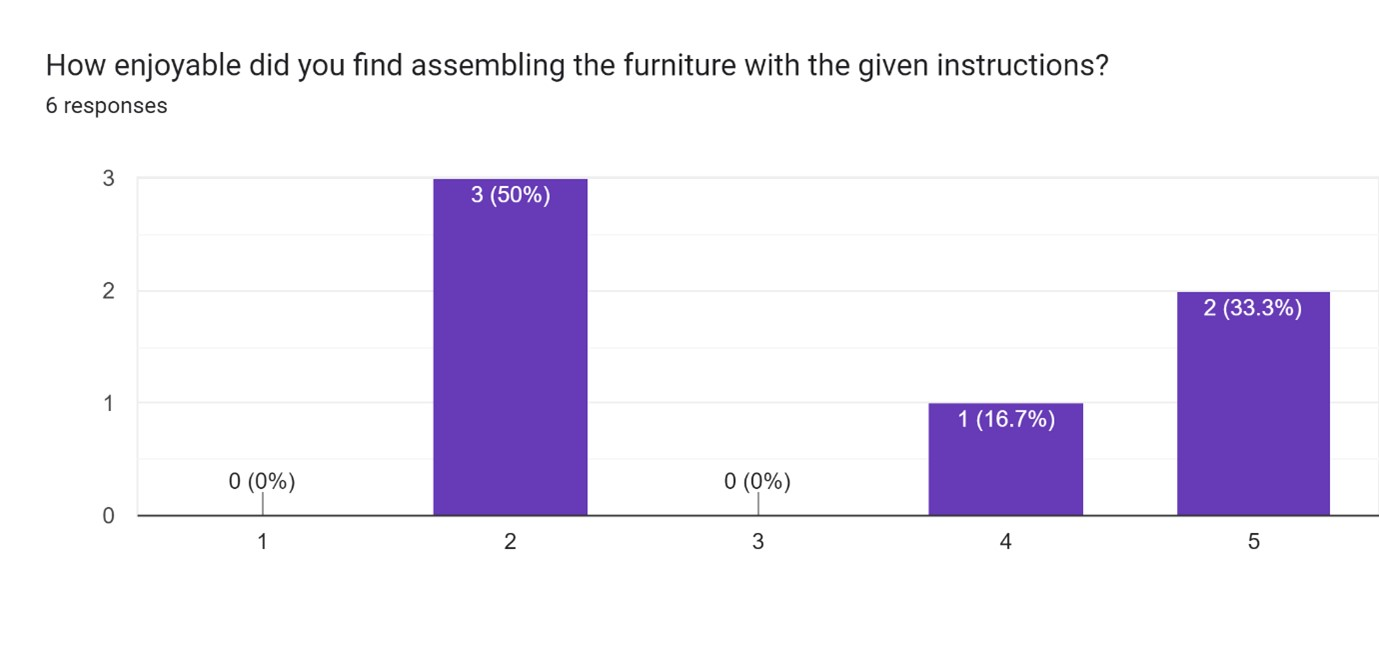
\includegraphics[width=0.5\linewidth]{dissertation//images/surveyEnjoyable.jpg}
    \caption{The results for the survey question, 'How enjoyable did you find assembling the furniture with the given instructions?' Results are on a scale from 'not enjoyable' to 'very enjoyable'.}
    \label{fig:surveyEnjoyable}
\end{figure}

Figure \ref{fig:surveyEnjoyable} shows a split in how much users enjoyed assembling the furniture with their given instructions. The users that gave the score of three were all the participants that used the tracking instructions.

\begin{figure}[hbt!]
    \centering
    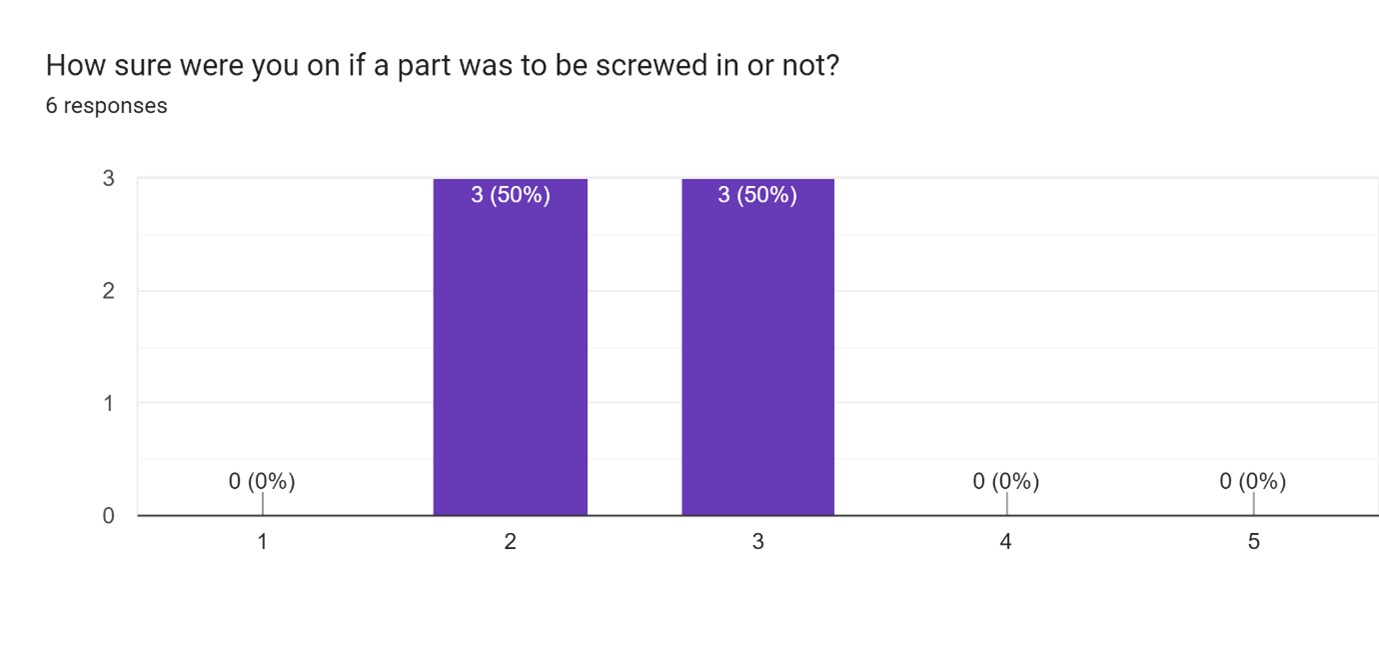
\includegraphics[width=0.5\linewidth]{dissertation//images/surveyScrew.jpg}
    \caption{The results for the survey question, 'How sure were you on if a part was to be screwed in or not?' Results are on a scale from 'not sure' to 'very sure'.}
    \label{fig:surveyScrew}
\end{figure}

Figure \ref{fig:surveyScrew} shows that participants generally gave a low score to how sure they were when to screw in a part. This matches comments from participants about the screw indicator not being very clear.

\subsection{Hololens Related Issues}

There were a selection of difficulties involving the Hololens that arose during the experiment.

Participants in the tracking group reported that the program was becoming slower as the steps progressed. Objects were losing positioning and frames were becoming choppy. The slow performance led to voice commands taking a while to respond. This meant that participants sometimes would say the command more than once which resulted them skipping steps without realising. Eventually the application would stop tracking and responding to voice commands altogether, which meant that the process had to be restarted and brought back to the correct step.

Another issue related to the Hololens was that there was a participant who wore glasses during the experiment. They reported issues that no other participant reported. They said they were experiencing 'double vision' and that using the headset was making them feel sick after a while.

\section{Discussion}

The research aimed to prove that AR instructions could offer a better experience for users than paper instructions. The experiment compared two versions of AR instructions against paper instructions, animated instructions and object tracking instructions. 

The nature of the issues in the paper and animated instructions were mostly very different. Issues in the tracking instructions were generally similar to the animated instructions. The exception to this being in part location. This emphasises how successful the animations were in highlighting locations of parts. However it is difficult to draw comparisons and evaluate the true effectiveness of them due to the tracking and technical difficulties encountered during testing. Tracking proved to be very tedious to use and attempting to use it severely decreased participant enjoyment. Despite this, due to the similarity to the animation instructions, the results help to highlight some of the benefits and downfalls of using the Hololens and AR instructions.

Paper instructions faced the lowest number of issues with part identification. This means that 3D models in an AR context may not be as useful to identify parts as may be expected. There are a few possible explanations for this. Parts appearing slightly transparent in the view of the Hololens might make it more difficult to make out their form. Without accurate shading it can be hard to identify features such as holes and grooves. The paper instructions have hard and bold outlines showing off every detail of the part which makes it clear to the user what features they are looking for.

One issue that was consistent across all forms of instructions was trouble with finding the correct orientation of parts. In the paper instructions, this could be explained by the fact that users are required to mentally rotate the parts to properly understand. As for the AR instructions, the transparency of parts could be the cause of the issue. For example, in thin pieces with holes, the holes would be visible on both sides which could cause confusion about which way it is facing. 

One of the biggest issues participants found with the paper instructions was finding the correct location for obscured parts in the pictures. This issue appeared every time there was a part which was not fully visible in the instructions which made it a fairly consistent issue. This is different to the animated instructions in which the most detrimental errors came in unique situations. Multiple participants in the animation group encountered similar issues when reaching a new type of step or in attempting to use a new feature. An exception to this was part identification issues but these issues were generally inconsequential. 

This theme matches what was shown in the plotted data. Figure \ref{fig:stepScores} shows a pattern of the number of issues decreasing quickly over time for animation and tracking instructions compared to the issues staying at a relatively consistent level for paper instructions. Using instructions on the Hololens was completely new to participants. Due to this there was a learning curve to completing tasks with them. When participants did not understand something, it often led to issues. As the process went on, participants started to gain a better understanding of how the system worked. It makes sense that the number of issues had with the AR instruction would start higher than the paper instructions as participants had all used them in some form before. There was no need for participants to spend time trying to understand what the paper instructions were communicating. The level of difficulty stays around this level as the AR level decreases which suggests there could be a higher baseline difficulty to using paper instructions than AR. Issues people have with paper instructions are generally issues they will keep having throughout.

These patterns, combined with the lower average error scores, prove that AR instructions are capable of offering users an improved experience over paper instructions. However, the user interface and guidance would need to be improved for users to get past the learning curve without outside assistance.

Another aim of the research was to highlight the advantages of using AR as a form of flatpack furniture assembly instructions.

One of the advantages shown from the research is the ability for the user to move around the instructions in 3D space. Participants were able to solve many of their issues by getting a different perspective of the step. 

Animations were very effective at communicating the location of parts to users. The part flying through 3D space along a recommended path helps to draw the eye towards the correct location, rather than them having to find it themselves.

Another advantage AR provides is the ability to place useful information and items in people's perspective. Participants made use of the arrow pointing to the next step multiple times to avoid getting lost. They also commented about how useful they found the name of the current part appearing on the screen to be.

Lastly, a common theme from participants that used the animation instructions was that it was quite an enjoyable experience. Using an AR implementation of instructions may offer a fun alternative to assembling flatpack furniture.

\section{Limitations}
\label{sec:exLimitations}

There were aspects to this experiment which hindered its overall effectiveness. Firstly, with only one assessor reviewing assembly task, it is difficult to mitigate bias in selecting when something should be noted. If a participant said nothing but appeared to be having difficulty, this was noted. Having more than one assessor to agree on what counts as an issue would help to reduce bias in the results.

With a sample size of nine participants, displaying data in the form of charts could be misleading. Outliers can have a big impact on the appearance of the results. A larger sample size or less focus on quantitative data could reduce this issue.

Each set of instructions were only tested on one piece of furniture. Instructions may perform differently on different complexities of assembly task. There may be other types of steps which are not covered in the furniture used in this task. It could be helpful to repeat the experiment for different assembly tasks.

Results were limited by the conditions of the environment the tests were carried out in. The room was very warm which made participants uncomfortable and contributed to the Hololens overheating. This led to many of the issues with the performance of the tracking instructions. A more comfortable environment would suit this experiment as it takes a long time to conduct and using the Hololens in heat for a long time causes it issues.

%==================================================================================================================================
\chapter{Conclusion}  
\label{chap:conclusion}

This project has explored the effectiveness of using augmented reality instructions on a head mounted display over paper instructions to assemble flatpack furniture. It assessed the benefits of such a design for assembly instructions. After analysing a set of IKEA paper instructions to find what kind of information it communicates, an application was designed for the Hololens 2 to give assembly instructions. The system behind the application was designed to be expandable, meaning it could automatically work with any 3D model, as long as it had the correct file structure. Two methods of communicating instructions were chosen, object tracking and animation. Object tracking involved tracking the position and rotation of parts of the flatpack furniture in real time and using this information to confirm if a part was in the right spot. Animation showed the path that a part should take to be added to the furniture. 

The system was evaluated in a user study which compared both versions of the AR instructions to paper instructions. Participants were split into three groups, paper, animation and tracking. The study involved participants assembling a piece of furniture and thinking aloud at moments which they felt confused or like there was an issue. Along with this, any moments the participants appeared confused and any errors they made were recorded. The results found that the AR instructions offered a lower overall error rate which is consistent with previous research in the field \citep{Tang2004, yang_comparing_2020}. Participants using AR instructions consistently started with a high amount of errors, with this amount dropping off quickly as the instructions progressed. This suggests there was a learning curve to using these instructions that was not present in the paper instructions which had a more consistent error level. The cause of such a steep learning curve could be the lack of detailed user guidance and a clear user interface within the application.

When designing and implementing the application, most of the focus and work effort was placed on the tracking instructions. This is because it seemed like the better option for communicating the instructions and highlighting errors before they would happen. It used an unfamiliar package which required a lot of work and acquiring a license to set up. Animation was designed as a backup option to tracking. Despite this, the user study proved the animations to be more effective at communicating instructions and stopping errors than the tracking method. Using tracking alone, in it's current state, provided no real benefits over using animation which has become a surprise stand-out option.

\section{Future Work}

This project was not free from difficulties and limitations. The experiment design had limitations as described in section \ref{sec:exLimitations}. A big issue that hindered the development was the difficulty in acquiring a license for VisionLib which was explained in section \ref{sec:license}. These difficulties caused delay and multiple changes of direction in the development process. Once the license was fully acquired, development could begin properly but with significantly less time. This meant that certain parts of the application could not be as well developed as intended. In the design for the application, the indicator to tell a user when to screw a part was planned to be rotating arrows around the screw hole. This ended up being reduced to a text indicator on the screen. The consequences of this became clear when participants expressed difficulty with knowing when to screw parts or not. Another feature which could have been implemented better was the height setup of the camera. In the final product the camera starts at a predetermined height. Ideally the camera height would be editable in runtime to account for different heights of users. The issues described here could all be solved in any future research.

Many of the problems participants had with the AR instructions during the assembly task could be solved with an improved user interface and comprehensive user guidance being present in the application. This could be implemented using tutorials or tool tips during the instructions. A tutorial to explain to users the difference between a component and a part might help them to understand, when a component is completed and added to the assembly, why no new part is being added.

In it's current state, object tracking with VisionLib is not ready for the purposes of this research. While this is the case, image tracking with unique images being placed on parts could be a temporary solution. It may not be a feasible solution for a real product but it could act as a proof of concept for the idea of tracking validation. Accurate part tracking could help to solve the issues of part identification and orientation which were most common in the animation instructions. With unique images on each part, they can be used to validate the user has chosen correctly. It would also be able to validate when the part has been rotated and placed in the correct way.

Since the animation instructions were a bigger success than expected, they should be taken further. Animations could be combined with object tracking. Parts could animate until the application detects that a part has been placed correctly, at which point it could stop the animation and show that the part is correct. This takes advantage of the benefits of both tracking and animation.

A feature which could be helpful for users is an ability to declare the space they want to assemble the furniture. In the current application it is required that the user starts the application facing away from where they want the build space to be. The assembly process then requires a certain amount of space in this area which may not suit the space the user is in. Allowing users to adjust their available workspace would give them more freedom and likely improve the assembly experience.

Finally, due to a limitation in the Unity editor's serialisation system, part and component objects could not be put in a list together, even though they could be within scripts. This meant that the instruction setup within the editor did not work for furniture which require adding parts and components between each other. To deal with this, the order of instructions had to be hard coded into the script. In future, a custom editor should be set up to create a better experience when developing AR instructions for other pieces of furniture.

%==================================================================================================================================
%
% 
%==================================================================================================================================
%  APPENDICES  

\begin{appendices}

\chapter{Appendices}

Typical inclusions in the appendices are:

\begin{itemize}
\item
  Copies of ethics approvals (required if obtained)
\item
  Copies of questionnaires etc. used to gather data from subjects.
\item
  Extensive tables or figures that are too bulky to fit in the main body of
  the report, particularly ones that are repetitive and summarised in the body.

\item Outline of the source code (e.g. directory structure), or other architecture documentation like class diagrams.

\item User manuals, and any guides to starting/running the software.

\end{itemize}

\textbf{Don't include your source code in the appendices}. It will be
submitted separately.

\begin{table}[!ht]
    \centering
    \rowcolors{2}{}{gray!3}
    \begin{tabular}{@{}l|llllll@{}}
        \textbf{Part} & \textbf{Part Identification} & \textbf{Location} & \textbf{Orientation} & \textbf{Progression}  & \textbf{Error} & \textbf{Other} \\ \hline
        \textbf{1}  & ~ & ~ & ~ & ~ & ~ & ~ \\ 
        \textbf{2}  & ~ & ~ & ~ & ~ & ~ & ~ \\ 
        \textbf{3}  & ~ & ~ & ~ & ~ & ~ & ~ \\ 
        \textbf{4}  & ~ & ~ & ~ & ~ & ~ & ~ \\ 
        \textbf{5}  & ~ & ~ & ~ & ~ & ~ & ~ \\ 
        \textbf{6}  & ~ & ~ & ~ & ~ & ~ & ~ \\ 
        \textbf{7}  & ~ & ~ & ~ & ~ & ~ & ~ \\ 
        \textbf{8}  & ~ & ~ & ~ & ~ & ~ & ~ \\ 
        \textbf{9}  & ~ & ~ & ~ & ~ & ~ & ~ \\ 
        \textbf{10} & ~ & ~ & ~ & ~ & ~ & ~ \\ 
        \textbf{11} & ~ & ~ & ~ & ~ & ~ & ~ \\ 
        \textbf{12} & ~ & ~ & ~ & ~ & ~ & ~ \\ 
        \textbf{13} & ~ & ~ & ~ & ~ & ~ & ~ \\ 
        \textbf{14} & ~ & ~ & ~ & ~ & ~ & ~ \\ 
        \textbf{15} & ~ & ~ & ~ & ~ & ~ & ~ \\ 
        \textbf{16} & ~ & ~ & ~ & ~ & ~ & ~ \\ 
        \textbf{17} & ~ & ~ & ~ & ~ & ~ & ~ \\ 
        \textbf{18} & ~ & ~ & ~ & ~ & ~ & ~ \\ 
        \textbf{19} & ~ & ~ & ~ & ~ & ~ & ~ \\ 
        \textbf{20} & ~ & ~ & ~ & ~ & ~ & ~ \\ 
        \textbf{21} & ~ & ~ & ~ & ~ & ~ & ~ \\ 
        \textbf{22} & ~ & ~ & ~ & ~ & ~ & ~ \\ 
        \textbf{23} & ~ & ~ & ~ & ~ & ~ & ~ \\ 
        \textbf{24} & ~ & ~ & ~ & ~ & ~ & ~ \\ 
        \textbf{25} & ~ & ~ & ~ & ~ & ~ & ~ \\ 
        \textbf{26} & ~ & ~ & ~ & ~ & ~ & ~ \\ 
        \textbf{27} & ~ & ~ & ~ & ~ & ~ & ~ \\ 
        \textbf{28} & ~ & ~ & ~ & ~ & ~ & ~ \\ 
        \textbf{29} & ~ & ~ & ~ & ~ & ~ & ~ \\ 
        \textbf{30} & ~ & ~ & ~ & ~ & ~ & ~ \\ 
        \textbf{31} & ~ & ~ & ~ & ~ & ~ & ~ \\ 
        \textbf{32} & ~ & ~ & ~ & ~ & ~ & ~ \\ 
        \textbf{33} & ~ & ~ & ~ & ~ & ~ & ~ \\ 
        \textbf{34} & ~ & ~ & ~ & ~ & ~ & ~ \\ 
        \textbf{35} & ~ & ~ & ~ & ~ & ~ & ~ \\ 
        \textbf{36} & ~ & ~ & ~ & ~ & ~ & ~ \\ 
        \textbf{37} & ~ & ~ & ~ & ~ & ~ & ~ \\ 
        \textbf{38} & ~ & ~ & ~ & ~ & ~ & ~ \\ 
        \textbf{39} & ~ & ~ & ~ & ~ & ~ & ~ \\ 
        \textbf{40} & ~ & ~ & ~ & ~ & ~ & ~ \\ 
        \textbf{41} & ~ & ~ & ~ & ~ & ~ & ~ \\ 
        \textbf{42} & ~ & ~ & ~ & ~ & ~ & ~ \\ 
        \textbf{43} & ~ & ~ & ~ & ~ & ~ & ~ \\ 
        \textbf{44} & ~ & ~ & ~ & ~ & ~ & ~ \\ 
        \textbf{45} & ~ & ~ & ~ & ~ & ~ & ~ \\ 
        \textbf{46} & ~ & ~ & ~ & ~ & ~ & ~ \\ 
        \textbf{47} & ~ & ~ & ~ & ~ & ~ & ~ \\ 
        \textbf{48} & ~ & ~ & ~ & ~ & ~ & ~ \\ 
        \textbf{49} & ~ & ~ & ~ & ~ & ~ & ~ \\ 
        \textbf{50} & ~ & ~ & ~ & ~ & ~ & ~ \\ 
        \textbf{51} & ~ & ~ & ~ & ~ & ~ & ~ \\ 
        \textbf{52} & ~ & ~ & ~ & ~ & ~ & ~ \\ 
        \textbf{53} & ~ & ~ & ~ & ~ & ~ & ~ \\ 
        \textbf{54} & ~ & ~ & ~ & ~ & ~ & ~ \\ 
        \textbf{55} & ~ & ~ & ~ & ~ & ~ & ~ \\ 
        \textbf{56} & ~ & ~ & ~ & ~ & ~ & ~ \\ 
        \textbf{57} & ~ & ~ & ~ & ~ & ~ & ~ \\ 
        \textbf{58} & ~ & ~ & ~ & ~ & ~ & ~ \\ 
        \textbf{59} & ~ & ~ & ~ & ~ & ~ & ~ \\ 
    \end{tabular}
\end{table}

\end{appendices}

%==================================================================================================================================
%   BIBLIOGRAPHY   

% The bibliography style is abbrvnat
% The bibliography always appears last, after the appendices.

\bibliographystyle{abbrvnat}

\bibliography{l4proj}

\end{document}
